\documentclass[11pt]{article}
\usepackage{myz310e-notes}
\usepackage{needspace}
\hypersetup{pdftitle={Attention and transformers: alignment, self-attention and a first look inside},pdfauthor={Emre Onur Kahya},pdfsubject={MYZ 310E Machine Learning in Physics, Fall 2026, lecture note 15 (week 6)}}
\newcommand{\hv}{\vect{h}}
\newcommand{\sv}{\vect{s}}
\newcommand{\cv}{\vect{c}}
\newcommand{\qv}{\vect{q}}
\newcommand{\kv}{\vect{k}}
\newcommand{\vv}{\vect{v}}
\newcommand{\ev}{\vect{e}}
\newcommand{\uv}{\vect{u}}
\newcommand{\pv}{\vect{p}}
\newcommand{\yv}{\vect{y}}
\newcommand{\gv}{\vect{g}}
\newcommand{\zv}{\vect{z}}
\newcommand{\onev}{\vect{1}}
\newcommand{\valpha}{\vect{\alpha}}
\newcommand{\softmax}{\operatorname{softmax}}
\newcommand{\LN}{\operatorname{LN}}
\newcommand{\MLP}{\operatorname{MLP}}
\newcommand{\diag}{\operatorname{diag}}
\newcommand{\blank}{\texttt{-}}
\renewcommand{\floatpagefraction}{0.75}
\renewcommand{\SourceNote}{%
  \par\vfill{\footnotesize\color{mute}The selection and order of topics in this note follow the lecture on attention
  models of the course IFT~6135 \emph{Representation Learning} at Université de Montréal and Mila (slides by Dzmitry
  Bahdanau, edited by Aaron Courville). The text, examples, figures and exercises of this note are original. Figures are
  computed from synthetic data by \texttt{figures\_note15.py}, published with the sources of these notes.\par}}

\begin{document}
\NoteTitle{15}{6}{Attention and transformers:\\ alignment, self-attention and a first look inside}{Attention and transformers}{%
An encoder--decoder recurrent network (Note~14, Section~7) must squeeze a whole input sequence into one vector before it starts to
produce the output. \emph{Attention} removes this bottleneck: at every output step the decoder computes a fresh weighted
average of all encoder states, with weights that measure how relevant each input position is right now. This note
derives soft attention and its gradient, follows location-based windows, connectionist temporal classification and
hard attention trained with REINFORCE, and arrives at \emph{self-attention}, where a sequence attends to itself and
recurrence disappears. The transformer is assembled piece by piece, with its costs, followed by decoder-only language
models, the key--value cache and IO-aware attention. The last section opens the box: the residual stream, what attention
patterns do and do not tell, ablation, activation patching and probes --- the tools of the course project.}

\section{Why attention: the fixed-vector bottleneck}\label{sec:bottleneck}

Attention is a learned, input-dependent weighting: the model computes a probability distribution over the parts of its
input and reads mostly from where that distribution puts its mass. A translation model weights the source words while it
writes each target word (Sections~\ref{sec:soft} and~\ref{sec:location}); an image model weights regions of an image, and
may look at only one of them (Section~\ref{sec:hard}); in a transformer every position weights all the others, and this
\emph{self-attention} replaces recurrence and convolution (Sections~\ref{sec:transformer} and~\ref{sec:modern}); a memory
network weights the slots of a memory by how well they match a query. In every case the model chooses its own wiring
diagram afresh for each input.

\paragraph{The sequence-to-sequence setting} The encoder--decoder of Note~14, Section~7, models a conditional
distribution of an output sequence $\yv = (y_1, \dots, y_{T'})$ given an input sequence $\x = (\x_1, \dots, \x_T)$ of
another length~\cite{kalchbrenner2013,sutskever2014,cho2014}. An encoder RNN reads $\x$, its final state $\vv$ (called
the context vector $\vect{s}$ in Note~14) is the only link to the decoder, and the decoder generates
\begin{equation}\label{eq:seq2seq}
  p(\yv \mid \x) = \prod_{i=1}^{T'} p(y_i \mid \vv, y_1, \dots, y_{i-1})
\end{equation}
token by token. In this note \emph{context vector} means instead the summary $\cv_i$ that attention recomputes at every
output step.

\paragraph{Two problems} Note~14, Section~11, lists the fixed-size bottleneck and the long paths among the limits of
recurrence. Here we make both quantitative.
\begin{itemize}
\item \emph{A bottleneck of fixed width.} However long the sentence, the decoder sees only the $d$ numbers of $\vv$. With
  $d = 1000$, a sentence of 50 words gets 20 numbers per word, a paragraph of 500 words only two.
\item \emph{Long paths.} The information about $\x_j$ reaches output step $i$ only after passing through $T - j$ encoder
  steps and $i$ decoder steps, and the gradient travels the same path backwards. Note~14, Section~4, showed that gradients
  through many recurrent steps vanish or explode; a path of length $T - j + i$ makes the first words of a long sentence the
  hardest to learn from.
\end{itemize}
Bahdanau, Cho and Bengio measured the effect directly: the translation quality of an RNN encoder--decoder fell
steadily with the length of the source sentence, while the same model with attention kept its quality on long
sentences~\cite{bahdanau2015}.

\begin{keyidea}
Instead of one summary $\vv$, keep all encoder states $\hv_1, \dots, \hv_T$, and let the decoder compute at each step $i$
a new summary $\cv_i = \sum_j \alpha_{ij}\hv_j$, with weights $\alpha_{ij} \ge 0$, $\sum_j \alpha_{ij} = 1$, that depend on
what the decoder needs at that step. The memory grows with the input, and every input position is connected to every
output step by a path of length two (encoder state $\to$ context $\to$ decoder state).
\end{keyidea}

\section{Soft content-based attention}\label{sec:soft}

\subsection{Context vectors and alignment weights}\label{sec:context}

Let $\hv_1, \dots, \hv_T \in \R^{d_h}$ be the encoder states and $\sv_i \in \R^{d_s}$ the decoder state from which $y_i$
is predicted (it has already read $y_{i-1}$). In the attention model of Bahdanau, Cho and Bengio~\cite{bahdanau2015} the decoder computes, at output
step $i$,
\begin{align}
  e_{ij} &= a(\sv_{i-1}, \hv_j), \qquad j = 1, \dots, T, \label{eq:score}\\
  \alpha_{ij} &= \frac{\exp(e_{ij})}{\sum_{k=1}^{T}\exp(e_{ik})}, \label{eq:alpha}\\
  \cv_i &= \sum_{j=1}^{T}\alpha_{ij}\,\hv_j , \label{eq:context}
\end{align}
and then uses the \emph{context vector} (or \emph{glimpse}) $\cv_i$ in place of the fixed $\vv$:
\[
  \sv_i = f(\sv_{i-1}, y_{i-1}, \cv_i), \qquad p(y_i \mid y_{<i}, \x) = \softmax\big(o(\sv_i, y_{i-1}, \cv_i)\big),
\]
with $f$ a GRU or LSTM update (Note~14, Sections~5 and~6) and $o$ a small output network. The \emph{score} or \emph{alignment model}
$a$ measures how well the input around position $j$ matches what the decoder is about to produce; the softmax
\eqref{eq:alpha} (Note~9, Section~4.4) turns the scores into a probability distribution over input positions; and the
context is the expectation of the encoder state under that distribution. Figure~\ref{fig:attstep} draws one step.

\begin{figure}[htbp]
\centering
\begin{tikzpicture}[x=1cm,y=1cm,font=\small,
  st/.style={draw=indigo,fill=indigo!6,minimum width=0.85cm,minimum height=0.6cm,inner sep=1pt},
  dec/.style={draw=teal,fill=teal!8,minimum width=0.95cm,minimum height=0.6cm,inner sep=1pt}]
  \foreach \j/\w in {1/0.4,2/0.6,3/2.2,4/1.0,5/0.4} {
    \node[st] (h\j) at (1.35*\j,0) {$\hv_{\j}$};
    \node[font=\scriptsize,color=mute] at (1.35*\j,-0.62) {$\x_{\j}$};
    \draw[-{Latex[length=1.6mm]},color=amber,line width=\w pt] (h\j.north) -- (4.05,1.55);
  }
  \node[circle,draw=amber,fill=amber!10,inner sep=1pt,minimum size=0.55cm] (c) at (4.05,1.8) {$\cv_i$};
  \node[font=\scriptsize,color=amber,anchor=west] at (6.25,0.75) {weights $\alpha_{ij}$};
  \node[dec] (s0) at (2.2,3.0) {$\sv_{i-1}$};
  \node[dec] (s1) at (5.9,3.0) {$\sv_i$};
  \node[font=\scriptsize] (y0) at (2.2,4.0) {$y_{i-1}$};
  \node[font=\scriptsize] (y1) at (5.9,4.0) {$y_i$};
  \draw[-{Latex[length=1.6mm]}] (s0) -- (s1);
  \draw[-{Latex[length=1.6mm]}] (c) -- (s1);
  \draw[-{Latex[length=1.6mm]}] (s1) -- (y1);
  \draw[-{Latex[length=1.6mm]}] (s0) -- (y0);
  \draw[-{Latex[length=1.6mm]}] (y0) -- (s1);
  \draw[-{Latex[length=1.6mm]},dashed,color=mute] (s0.south) to[out=-90,in=90] node[left,font=\scriptsize,pos=0.45] {scores $e_{ij}$} (h2.north west);
  \node[font=\scriptsize,color=mute,align=left,anchor=west] at (7.3,0) {bidirectional\\encoder states};
  \node[font=\scriptsize,color=mute,align=left,anchor=west] at (7.3,3.0) {decoder RNN};
\end{tikzpicture}
\caption{One decoder step with soft attention. The previous decoder state $\sv_{i-1}$ is compared with every encoder
state (dashed arrow); the softmax of the scores gives the weights $\alpha_{ij}$ (line widths); the weighted average
$\cv_i$ enters the update of the decoder state together with $\sv_{i-1}$ and $y_{i-1}$.}
\label{fig:attstep}
\end{figure}

\paragraph{Why a bidirectional encoder} The state $\hv_j$ should describe the input \emph{around} position $j$, not just
the prefix $\x_1, \dots, \x_j$. Bahdanau et al.\ therefore concatenate the states of a forward and a backward RNN,
$\hv_j = [\overrightarrow{\hv}_j; \overleftarrow{\hv}_j]$ (Note~14, Section~9). With a forward RNN alone, $\hv_j$ would know nothing
about the words after $j$, and an early word whose translation depends on a later one could not be matched correctly.
Plain word embeddings, with no recurrence at all, would be worse still: the score could then only compare the decoder
state with a single word out of context.

\paragraph{Soft attention is a differentiable lookup} Everything in \eqref{eq:score}--\eqref{eq:context} is smooth, so the
alignment is learned by backpropagation from translation pairs alone; nobody tells the model which words correspond.

\subsection{Scoring functions}\label{sec:scores}

The original paper used a one-hidden-layer network for $a$, the \emph{additive} (or concat) score. Luong, Pham and
Manning compared simpler alternatives~\cite{luong2015}, and the transformer added a scaled version of the dot product. With
$\sv$ the decoder state and $\hv$ an encoder state:
\begin{center}\small
\begin{tabular}{@{}llll@{}}
\toprule
name & score $a(\sv, \hv)$ & parameters & cost per pair \\
\midrule
additive~\cite{bahdanau2015} & $\vect{w}_a\T\tanh(W_a\sv + U_a\hv)$ & $d_a(d_s + d_h + 1)$ & $O(d_a)$ after precomputing $U_a\hv$ \\
dot~\cite{luong2015} & $\sv\T\hv$ & none ($d_s = d_h = d$) & $O(d)$ \\
bilinear (``general'')~\cite{luong2015} & $\sv\T M\hv$ & $d_sd_h$ & $O(d_h)$ after precomputing $M\T\sv$ \\
scaled dot~\cite{vaswani2017} & $\sv\T\hv/\sqrt{d}$ & none ($d_s = d_h = d$) & $O(d)$ \\
\bottomrule
\end{tabular}
\end{center}
Here $d = d_s = d_h$ wherever the two states must have the same width. The dot product needs no parameters but requires the decoder and encoder states to live in the same space; the bilinear
form learns a map between the two spaces; the additive score is the most flexible and the slowest. Section~\ref{sec:sdpa}
explains the factor $1/\sqrt{d}$.

\begin{worked}{1. Three scores on three encoder states}
Let $T = 3$ and $d = 2$ with $\hv_1 = (1, 0)$, $\hv_2 = (0, 1)$, $\hv_3 = (1, 1)$ and the decoder state $\sv = (1, 2)$.
\emph{Dot product:} $e = (1, 2, 3)$. Then $e^{e_j} = (2.718, 7.389, 20.086)$ with sum $30.193$, so
\[
  \valpha = (0.090, 0.245, 0.665), \qquad \cv = 0.090\,\hv_1 + 0.245\,\hv_2 + 0.665\,\hv_3 = (0.755, 0.910) .
\]
\emph{Scaled dot product:} $e/\sqrt2 = (0.707, 1.414, 2.121)$ gives the flatter $\valpha = (0.140, 0.284, 0.576)$ and
$\cv = (0.716, 0.860)$.
\emph{Bilinear} with $M = \big(\begin{smallmatrix} 0 & 1 \\ 1 & 0 \end{smallmatrix}\big)$, which swaps the two
components: $e = (2, 1, 3)$ and $\valpha = (0.245, 0.090, 0.665)$; the learned matrix changed which state ranks second.
\emph{Additive} with $W_a = U_a = I$ and $\vect{w}_a = (1, 1)$: the hidden vectors are $\tanh(\sv + \hv_j) =
(0.964, 0.964)$, $(0.762, 0.995)$, $(0.964, 0.995)$, so $e = (1.928, 1.757, 1.959)$ and
$\valpha = (0.348, 0.293, 0.359)$. The $\tanh$ is close to saturation, the scores barely differ and the weights are almost
uniform: the scale of the parameters matters as much as the form of the score.
\end{worked}

\subsection{The gradient through attention}\label{sec:attgrad}

Backpropagation (Note~12, Section~3) needs the derivatives of \eqref{eq:alpha} and \eqref{eq:context}. Suppose the
gradient $\bar{\cv} = \partial\ell/\partial\cv$ of the loss with respect to the context has arrived from above (we drop the
output index $i$).

\emph{Through the weighted sum.} Since $\cv = \sum_j \alpha_j\hv_j$,
\begin{equation}\label{eq:gradvalue}
  \frac{\partial\ell}{\partial\alpha_j} = \bar{\cv}\T\hv_j \eqqcolon g_j, \qquad
  \frac{\partial\ell}{\partial\hv_j}\Big|_{\text{via }\cv} = \alpha_j\,\bar{\cv} .
\end{equation}
Each encoder state receives the incoming gradient scaled by its own weight: positions the decoder did not look at
receive almost nothing through this path.

\emph{Through the softmax.} With $\alpha_j = e^{e_j}/\sum_k e^{e_k}$, the derivative is $\partial\alpha_j/\partial e_m =
\alpha_j(\delta_{jm} - \alpha_m)$, that is, the Jacobian is $\diag(\valpha) - \valpha\valpha\T$ (Note~12, Section~2). Hence
\begin{equation}\label{eq:gradscore}
  \frac{\partial\ell}{\partial e_m} = \sum_j g_j\,\alpha_j(\delta_{jm} - \alpha_m) = \alpha_m\big(g_m - \bar g\big),
  \qquad \bar g = \sum_j \alpha_j g_j .
\end{equation}
The gradient of a score is the weight of that position times how much more its value $\hv_m$ increases the loss than the
current average $\bar g$ does; descent lowers that score when $g_m > \bar g$ and raises it when $g_m < \bar g$. Three
consequences follow. The score gradients sum to zero, because adding a constant to all
scores changes nothing. A position with $\alpha_m \approx 0$ gets almost no gradient, so a position the model ignores
can be difficult to discover again. And if the softmax is saturated, $\valpha \approx$ one-hot, then $\alpha_m(g_m - \bar g)
\approx 0$ for every $m$: a saturated attention distribution stops learning, one reason, at initialisation, for the scaling
of Section~\ref{sec:sdpa}. Finally the score gradients flow into the parameters of $a$ and, a second time, into $\hv_j$ and $\sv$.

\begin{worked}{2. Backward pass through Worked example~1}
Take the dot-product weights $\valpha = (0.090, 0.245, 0.665)$ and the loss $\ell = \uv\T\cv$ with $\uv = (1, -1)$, so
$\bar{\cv} = \uv$. Then $g_j = \uv\T\hv_j = (1, -1, 0)$ and $\bar g = 0.090 - 0.245 = -0.155$, and by \eqref{eq:gradscore}
\[
  \frac{\partial\ell}{\partial\ev} = \big(0.090 \cdot 1.155,\ 0.245 \cdot (-0.845),\ 0.665 \cdot 0.155\big)
  = (0.104, -0.207, 0.103) ,
\]
which sums to zero. Gradient descent ($\ev \gets \ev - \eta\,\partial\ell/\partial\ev$) would lower the scores of $\hv_1$
and $\hv_3$ and raise that of $\hv_2$, the only state whose value decreases the loss ($g_2 = -1 < \bar g$). Through \eqref{eq:gradvalue} the encoder states receive $\alpha_j\uv$: $(0.090, -0.090)$,
$(0.245, -0.245)$ and $(0.665, -0.665)$. Central differences with step $10^{-6}$ (Note~12, Section~4) reproduce the three
score gradients to six digits.
\end{worked}

\subsection{The algorithm and its cost}\label{sec:attalg}

Algorithm~\ref{alg:attdec} computes one decoder step with additive attention. The products $U_a\hv_j$ do not depend on
the decoder and are computed once per input sequence.

\begin{algorithm}[htbp]
\caption{One decoder step of an RNN encoder--decoder with additive attention}\label{alg:attdec}
\begin{algorithmic}[1]
\Require encoder states $H = [\hv_1, \dots, \hv_T]\T \in \R^{T \times d_h}$; precomputed $P = HU_a\T \in \R^{T \times d_a}$;
  previous state $\sv_{i-1}$ and token $y_{i-1}$; parameters $W_a, \vect{w}_a$, decoder update $f$ and output map $o$
\Function{AttentionStep}{$\sv_{i-1}, y_{i-1}$; $H, P$}
  \State $\vect{r} \gets W_a\sv_{i-1}$ \Comment{$O(d_ad_s)$}
  \State $e_j \gets \vect{w}_a\T\tanh(\vect{r} + P_{j,:})$ for $j = 1, \dots, T$ \Comment{add a vector to a matrix, $O(Td_a)$}
  \State $e^* \gets \max_j e_j$; \ $\alpha_j \gets \exp(e_j - e^*) / \sum_k \exp(e_k - e^*)$ \Comment{stable softmax}
  \State $\cv_i \gets H\T\valpha$ \Comment{vector--matrix product, $O(Td_h)$}
  \State $\sv_i \gets f(\sv_{i-1}, y_{i-1}, \cv_i)$ \Comment{GRU or LSTM update}
  \State \Return $\sv_i$, $p(y_i \mid \cdot) = \softmax\big(o(\sv_i, y_{i-1}, \cv_i)\big)$, and $\valpha$ for inspection
\EndFunction
\end{algorithmic}
\end{algorithm}

\begin{runtime}{attention decoder (Algorithm~\ref{alg:attdec})}
\emph{Per input}: $O(Td_hd_a)$ once for $P$. \emph{Per output step}: $O(d_ad_s)$ for $W_a\sv$, $O(Td_a)$ for the scores,
$O(T)$ for the softmax and $O(Td_h)$ for the context, on top of the $O(d_s^2 + d_sd_h)$ recurrent update and the
$O(d_sV)$ output softmax over a vocabulary of size $V$. \emph{Per sequence pair}: $O\big(TT'(d_a + d_h)\big)$ for attention,
quadratic in the lengths, but every step is a vector--matrix product that runs fast on a GPU. \emph{Memory}: $O(Td_h)$ for
the encoder states, and the $T \times T'$ weights kept for the backward pass. \emph{Training} with teacher forcing
(Note~14, Section~7) costs about three times the forward pass; \emph{prediction} with beam width $B$ costs $B$ times a greedy decode.
\end{runtime}

\subsection{Reading alignments}\label{sec:alignvis}

The matrix of weights $\alpha_{ij}$, with output steps as rows and input positions as columns, can be drawn as an image.
Between languages with a similar word order it is close to diagonal. Figure~\ref{fig:align} shows a pair with a
different order: English ``I read the red book'' and Turkish ``kırmızı kitabı okudum''. The verb moves to the end, and the
subject ``I'' and the article ``the'' have no word of their own: they become the personal ending of ``okudum'' and the
accusative ending of ``kitabı'', which marks a definite object. A row
with one dominant entry is a one-to-one correspondence. A row with two large entries is a Turkish word that does the work
of two English words, and the order of the large entries from row to row shows the reordering.
Section~\ref{sec:patterns} will qualify how much such pictures explain.

\begin{figure}[htbp]
\centering
\begin{tikzpicture}[x=1.25cm,y=0.62cm,font=\small]
  \foreach \c/\w in {1/I,2/read,3/the,4/red,5/book} \node[anchor=south] at (\c,0.55) {\w};
  \foreach \r/\w in {1/kırmızı,2/kitabı,3/okudum} \node[anchor=east] at (0.45,-\r+1) {\w};
  \foreach \r/\c/\a in {1/1/0.04,1/2/0.05,1/3/0.05,1/4/0.76,1/5/0.10,
                        2/1/0.04,2/2/0.04,2/3/0.22,2/4/0.07,2/5/0.63,
                        3/1/0.25,3/2/0.56,3/3/0.05,3/4/0.06,3/5/0.08} {
    \pgfmathsetmacro{\shade}{100*\a}
    \fill[indigo!\shade!white] (\c-0.5,-\r+1.5) rectangle (\c+0.5,-\r+0.5);
    \pgfmathparse{\a>0.5 ? 1 : 0}
    \ifnum\pgfmathresult=1 \node[color=white,font=\scriptsize] at (\c,-\r+1) {\a};
    \else \node[font=\scriptsize] at (\c,-\r+1) {\a}; \fi
  }
  \draw[color=mute] (0.5,0.5) rectangle (5.5,-2.5);
\end{tikzpicture}
\caption{Illustrative attention weights for translating ``I read the red book'' into Turkish (rows: output words; columns:
input words; darker means larger). The weights are softmaxes of hand-chosen scores, not the output of a trained model.}
\label{fig:align}
\end{figure}

\paragraph{Strengths and weaknesses} The length experiment of Bahdanau et al.\ quoted in Section~\ref{sec:bottleneck} is
the main argument for soft attention. Its weakness shows when input and output are aligned \emph{monotonically}, as speech
frames and the letters of the transcript: content alone is then a weak guide (two occurrences of the same sound look alike,
and the model can jump back or skip), and the cost $O(TT')$ is a burden for inputs of thousands of steps.
Sections~\ref{sec:location} and~\ref{sec:flash} return to these problems.

\begin{physics}{attention weights are Boltzmann weights}
Note~11, Section~2 (physics box), read the softmax as a Boltzmann distribution with energies $E_j = -e_j$, and Note~5,
Section~3.3, read the factor $\sqrt{d_k}$ of Section~\ref{sec:sdpa} as a temperature. With $\alpha_j = e^{e_j/\tau}/Z$, the
context vector is the thermal average $\langle\hv\rangle$, and the free energy $F = -\tau\log Z$ has
$-\partial F/\partial e_m = \alpha_m$. New here is the gradient \eqref{eq:gradscore} read as a fluctuation formula: $\partial\langle g\rangle/\partial e_m = \alpha_m(g_m - \langle g\rangle)/\tau$, which reduces to
\eqref{eq:gradscore} at $\tau = 1$, is the covariance of $g$ with the indicator of position $m$, divided by $\tau$, as
derivatives of thermal averages with respect to couplings are connected correlations. A frozen system has no
fluctuations, hence no gradient --- the statistical-mechanics reading of a saturated softmax.
\end{physics}

\section{Location-based attention and monotonic alignment}\label{sec:location}

In content-based attention the weights depend on the \emph{content} at each input position. In \emph{location-based}
attention they depend on \emph{where} the model attended before: the new weights are computed relative to the old ones. The
idea is older than content-based attention; it was introduced by Graves for handwriting
synthesis~\cite{graves2013}, where a network must write a given text letter by letter and must move through the text in
order.

\subsection{A Gaussian window that only moves forward}\label{sec:graves}

Let $\vect{\chi}_1, \dots, \vect{\chi}_U$ be the one-hot vectors of the $U$ characters to be written. (We follow Graves's notation: in this subsection $\hv_t$ is
the state of the network that writes, and $\alpha$, $\beta$, $\kappa$ are window parameters, not attention weights.) At each
pen step $t$ the network's
hidden state $\hv_t$ emits, through a linear layer, $3K$ numbers $(\hat{\alpha}_t, \hat{\beta}_t, \hat{\kappa}_t) \in \R^{3K}$ and
defines a mixture of $K$ Gaussian bumps over character positions $u$:
\begin{equation}\label{eq:window}
  \phi(t, u) = \sum_{k=1}^{K}\alpha_t^k\exp\!\big(-\beta_t^k(\kappa_t^k - u)^2\big), \qquad
  \vect{w}_t = \sum_{u=1}^{U}\phi(t, u)\,\vect{\chi}_u ,
\end{equation}
with
\begin{equation}\label{eq:windowparams}
  \alpha_t^k = \exp(\hat{\alpha}_t^k), \qquad \beta_t^k = \exp(\hat{\beta}_t^k), \qquad
  \kappa_t^k = \kappa_{t-1}^k + \exp(\hat{\kappa}_t^k) .
\end{equation}
The \emph{window vector} $\vect{w}_t$, a soft bag of the characters under the window, is passed to the other layers of the network and, at the next
step, back to the layer that computes the window. The amplitude $\alpha$ sets the importance of a bump, $\beta$ its sharpness (width about $1/\sqrt{\beta}$), and
$\kappa$ its centre. Because the centre advances by the positive amount $\exp(\hat{\kappa}_t^k)$, the window can only slide
forwards: the alignment is monotonic by construction. The weights are not normalised; the network can switch the window off
by making all amplitudes small.

\begin{worked}{3. A window sliding over five characters}
Take $K = 1$, $\alpha = 1$, $\beta = 2$, $\kappa_0 = 0$, and offsets $\exp(\hat{\kappa}_t) = 1.0, 0.6, 0.6, 1.2$ for
$t = 1, \dots, 4$, so that $\kappa_t = 1.0, 1.6, 2.2, 3.4$. For the positions $u = 1, \dots, 5$,
$\phi(t, u) = \exp(-2(\kappa_t - u)^2)$ gives
\begin{center}\small
\begin{tabular}{@{}cccccc@{}}
\toprule
$t$ ($\kappa_t$) & $u = 1$ & $u = 2$ & $u = 3$ & $u = 4$ & $u = 5$ \\
\midrule
1 (1.0) & 1.000 & 0.135 & 0.000 & 0.000 & 0.000 \\
2 (1.6) & 0.487 & 0.726 & 0.020 & 0.000 & 0.000 \\
3 (2.2) & 0.056 & 0.923 & 0.278 & 0.002 & 0.000 \\
4 (3.4) & 0.000 & 0.020 & 0.726 & 0.487 & 0.006 \\
\bottomrule
\end{tabular}
\end{center}
For example $\phi(2, 1) = e^{-2 \cdot 0.36} = e^{-0.72} = 0.487$. If the five characters are all different,
$\vect{w}_t$ simply lists these weights, one per letter; a repeated letter would collect the sum of its weights. The writer dwells on characters~1 and~2 for three steps (a letter takes several pen strokes), then
moves on; the large offset at $t = 4$ skips ahead by more than a character. The window never moves back.
\end{worked}

Figure~\ref{fig:window} follows a window with two components over forty-six steps of a thirty-character text, with random
offsets of mean about $0.6$ characters per step: the bright band climbs monotonically, faster when the offsets are larger.

\begin{figure}[htbp]
\centering
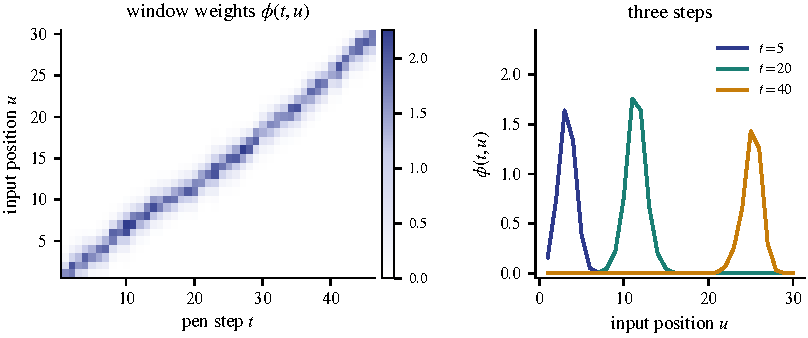
\includegraphics[width=0.86\linewidth]{figures/n15_window.pdf}
\caption{A Gaussian-mixture window \eqref{eq:window} with $K = 2$ moving along $U = 30$ characters. Left: $\phi(t, u)$ for
46 steps with random positive offsets. Right: the window at three steps. The alignment is monotonic because the centres
can only increase.}
\label{fig:window}
\end{figure}

\begin{algorithm}[htbp]
\caption{Gaussian-mixture window (one step)}\label{alg:window}
\begin{algorithmic}[1]
\Require hidden state $\hv_t$; previous centres $\vect{\kappa}_{t-1} \in \R^K$; character vectors $\vect{\chi}_1, \dots, \vect{\chi}_U$;
  output layer $W, \vect{b}$
\Function{WindowStep}{$\hv_t, \vect{\kappa}_{t-1}$}
  \State $(\hat{\vect{\alpha}}, \hat{\vect{\beta}}, \hat{\vect{\kappa}}) \gets W\hv_t + \vect{b}$ \Comment{$3K$ numbers}
  \State $\vect{\alpha} \gets \exp(\hat{\vect{\alpha}})$; \ $\vect{\beta} \gets \exp(\hat{\vect{\beta}})$; \
    $\vect{\kappa}_t \gets \vect{\kappa}_{t-1} + \exp(\hat{\vect{\kappa}})$ \Comment{centres only move forward}
  \For{$u = 1, \dots, U$}
    \State $\phi_u \gets \sum_{k=1}^{K}\alpha^k\exp\big(-\beta^k(\kappa_t^k - u)^2\big)$
  \EndFor
  \State \Return $\vect{w}_t = \sum_u \phi_u\vect{\chi}_u$ and $\vect{\kappa}_t$
\EndFunction
\end{algorithmic}
\end{algorithm}

\begin{runtime}{Gaussian-mixture window}
\emph{Time}: $O(Kd_h)$ for the window parameters and $O(KU)$ for the weights per step; in practice only the few positions
within a handful of widths of each centre matter, so the cost can be cut to $O(K)$ per step with truncation. Over $T$ steps,
$O(T(Kd_h + KU))$, far less than content-based attention when $U$ is large. \emph{Memory}: $O(U)$ for the weights per step,
$O(TU)$ (or $O(TK)$ truncated) for training. The window adds only $3K(d_h + 1)$ parameters.
\end{runtime}

\paragraph{Variants} Content and location can be mixed. Chorowski et al.\ added to the content score a term computed by a
convolution of the previous alignment $\valpha_{i-1}$, so that the model knows where it looked last and prefers to move a
little forward; this made attention-based speech recognition work on long utterances~\cite{chorowski2015}. Other
variants keep a running summary of past alignments in a small recurrent network, a generalisation of that convolution, or
give every input position its own learned embedding so that keys can encode location, as memory networks do. A purely
location-based window, on the other hand, cannot repair its mistakes: if a jump such as the one at $t = 4$ in Worked example~3 skips a
character that still had to be written, it can never be undone, because the centres cannot move back.

\subsection{Connectionist temporal classification}\label{sec:ctc}

\emph{Connectionist temporal classification} (CTC)~\cite{graves2006} predates soft attention and is still widely used for
speech and handwriting recognition. It solves the monotonic alignment problem exactly, by summing over all alignments.

\paragraph{Paths and the collapse map} An RNN (or any network) reads the $T$ input frames and outputs at every frame a
distribution $y^t_k$ over the alphabet plus one extra symbol, the \emph{blank} ``\blank''. A sequence $\pi = (\pi_1, \dots,
\pi_T)$ of such symbols is a \emph{path}. The collapse map $\mathcal{B}$ first merges repeated symbols and then deletes
blanks: $\mathcal{B}(\texttt{aa-b}) = \mathcal{B}(\texttt{a-bb}) = \texttt{ab}$, while $\mathcal{B}(\texttt{a-a}) =
\texttt{aa}$ --- a blank is needed between two equal letters. The labelling $\vect{l}$ (which needs $T \ge |\vect{l}| + r$,
where $r$ is the number of adjacent equal labels in $\vect{l}$) gets the probability
\begin{equation}\label{eq:ctc}
  p(\vect{l} \mid \x) = \sum_{\pi \in \mathcal{B}^{-1}(\vect{l})} p(\pi \mid \x)
  = \sum_{\pi \in \mathcal{B}^{-1}(\vect{l})} \prod_{t=1}^{T} y^t_{\pi_t} .
\end{equation}
Each path is a monotonic \emph{hard} alignment of the label to the frames, and CTC marginalises over all of them. The
product form assumes that the symbols at different frames are conditionally independent given $\x$; the dependence between
output symbols comes only through the shared input. The RNN transducer of Graves removes this assumption by feeding the
previously emitted labels to a prediction network while keeping the monotonic sum over alignments~\cite{graves2012}.
Training maximises $\log p(\vect{l} \mid \x)$ (maximum likelihood, Note~2, Section~2.1).

\paragraph{The forward recursion} The number of paths grows exponentially with $T$, but monotonicity allows dynamic
programming. Insert blanks around and between the labels, $\vect{l}' = (\blank, l_1, \blank, l_2, \dots, l_{|\vect{l}|},
\blank)$, of length $S = 2|\vect{l}| + 1$, and let $\gamma_t(s)$ be the total probability of all path prefixes of length $t$
that end at position $s$ of $\vect{l}'$ and are consistent with it. A path may stay on the same symbol, advance by one, or
skip a blank between two \emph{different} labels:
\begin{equation}\label{eq:ctcfwd}
  \gamma_t(s) = y^t_{l'_s}\Big(\gamma_{t-1}(s) + \gamma_{t-1}(s - 1) + \ind{l'_s \ne \blank \text{ and } l'_s \ne l'_{s-2}}\,\gamma_{t-1}(s - 2)\Big),
\end{equation}
with $\gamma_1(1) = y^1_{\blank}$, $\gamma_1(2) = y^1_{l_1}$, and $\gamma_1(s) = 0$ otherwise. A complete path ends on the last
label or on the final blank: $p(\vect{l} \mid \x) = \gamma_T(S) + \gamma_T(S - 1)$. A backward recursion of the same form
gives the gradient, as in the forward--backward algorithm of hidden Markov models.

\begin{worked}{4. CTC on three frames}
Alphabet $\{\texttt{a}, \texttt{b}\}$ plus blank, $T = 3$ frames, label $\vect{l} = \texttt{ab}$. The network outputs
\begin{center}\small
\begin{tabular}{@{}lccc@{}}
\toprule
frame & $y_{\texttt{a}}$ & $y_{\texttt{b}}$ & $y_{\blank}$ \\
\midrule
1 & 0.6 & 0.1 & 0.3 \\
2 & 0.2 & 0.3 & 0.5 \\
3 & 0.1 & 0.6 & 0.3 \\
\bottomrule
\end{tabular}
\end{center}
\emph{By enumeration.} Five of the $27$ paths collapse to \texttt{ab}: \texttt{aab} ($0.6 \cdot 0.2 \cdot 0.6 = 0.072$),
\texttt{abb} ($0.108$), \texttt{ab-} ($0.054$), \texttt{a-b} ($0.180$) and \texttt{-ab} ($0.036$); the total is
$p(\texttt{ab} \mid \x) = 0.450$.
\emph{By the recursion} on $\vect{l}' = (\blank, \texttt{a}, \blank, \texttt{b}, \blank)$:
\begin{center}\small
\begin{tabular}{@{}lccccc@{}}
\toprule
& $\blank$ & \texttt{a} & $\blank$ & \texttt{b} & $\blank$ \\
\midrule
$\gamma_1$ & 0.300 & 0.600 & 0 & 0 & 0 \\
$\gamma_2$ & 0.150 & 0.180 & 0.300 & 0.180 & 0 \\
$\gamma_3$ & 0.045 & 0.033 & 0.144 & 0.396 & 0.054 \\
\bottomrule
\end{tabular}
\end{center}
For instance $\gamma_2(\texttt{b}) = 0.3\,(0 + 0 + 0.6) = 0.18$ uses the skip from \texttt{a} over the blank, and
$\gamma_3(\texttt{b}) = 0.6\,(0.18 + 0.30 + 0.18) = 0.396$. The answer $\gamma_3(4) + \gamma_3(5) = 0.396 + 0.054 = 0.450$ agrees.
The label \texttt{aa} has only one path of length three, \texttt{a-a}, with probability $0.6 \cdot 0.5 \cdot 0.1 = 0.03$.
\end{worked}

\begin{algorithm}[htbp]
\caption{CTC forward pass}\label{alg:ctc}
\begin{algorithmic}[1]
\Require per-frame distributions $y^t$ over the alphabet and blank, $t = 1, \dots, T$; label $\vect{l}$
\Function{CTCForward}{$y, \vect{l}$}
  \State $\vect{l}' \gets (\blank, l_1, \blank, \dots, l_{|\vect{l}|}, \blank)$; \ $S \gets 2|\vect{l}| + 1$
  \State $\gamma_1(1) \gets y^1_{\blank}$; \ $\gamma_1(2) \gets y^1_{l_1}$; \ $\gamma_1(s) \gets 0$ for $s > 2$
  \For{$t = 2, \dots, T$}
    \For{$s = 1, \dots, S$}
      \State $b \gets \gamma_{t-1}(s) + \gamma_{t-1}(s - 1)$ \Comment{stay or advance; $\gamma(0) = 0$}
      \If{$l'_s \ne \blank$ and $s > 2$ and $l'_s \ne l'_{s-2}$} $b \gets b + \gamma_{t-1}(s - 2)$ \Comment{skip a blank}
      \EndIf
      \State $\gamma_t(s) \gets y^t_{l'_s}\, b$
    \EndFor
  \EndFor
  \State \Return $\log\big(\gamma_T(S) + \gamma_T(S - 1)\big)$ \Comment{in practice: work with $\log\gamma$ and log-sum-exp}
\EndFunction
\end{algorithmic}
\end{algorithm}

\begin{runtime}{CTC loss}
\emph{Time}: $O(TS) = O(T|\vect{l}|)$ for the forward recursion and the same for the backward one, negligible next to the
network that produces the $y^t$. \emph{Memory}: $O(TS)$ for the table, needed by the backward pass. Products of many
probabilities underflow, so implementations work with logarithms (the log-sum-exp trick of Note~5, Section~3.3) or rescale
each row. \emph{Prediction}: the most likely labelling has no closed form; taking the most likely symbol at every frame and
collapsing (best-path decoding) costs $O(TV)$, and a prefix beam search with width $B$ is more accurate.
\end{runtime}

\paragraph{Comparison} The three mechanisms differ in what they assume. Content-based weights assume nothing about the
order of the alignment; a location-based window assumes that it is monotonic; CTC assumes in addition that the outputs
are conditionally independent, and in exchange computes the likelihood exactly. Each path of CTC is a hard alignment, one
label position per frame, yet the gradient is exact because the paths are summed rather than sampled: Worked example~4
computed exactly the sum that the sampling estimator of Section~\ref{sec:reinforce} would have to approximate.

\begin{modern}{speech recognition today}
Both lines are alive. Self-supervised speech encoders such as wav2vec~2.0 are fine-tuned for recognition with a CTC
output layer~\cite{baevski2020}, which keeps decoding simple and strictly monotonic. Whisper~\cite{radford2023} instead uses
a transformer encoder--decoder of the kind assembled in Section~\ref{sec:transformer}: the encoder reads a log-Mel
spectrogram, and the decoder attends to it with the cross-attention of Section~\ref{sec:threekinds} while generating text;
trained on a very large collection of weakly labelled audio, it transcribes and translates many languages.
\end{modern}

\section{Hard attention and glimpses}\label{sec:hard}

\subsection{A recurrent model of visual attention}\label{sec:ram}

A convolutional network (Note~13) processes the whole image at full resolution, and its cost grows with the number of
pixels. The eye works differently: only the fovea, about two degrees of the visual field, is sharp, so we scan a scene
with a few saccades per second and combine what each fixation reveals. The \emph{recurrent attention model} (RAM) of Mnih,
Heess, Graves and Kavukcuoglu~\cite{mnih2014} imitates this.
A \emph{glimpse sensor} extracts, around a location $\vect{l}_{t-1}$, a few patches of increasing size, all reduced to
the same small number of pixels, so that the centre is seen sharply and the surround coarsely. A \emph{glimpse network}
maps them and the location to features $\vect{g}_t$, and a \emph{core} RNN updates its state $\hv_t = f_h(\hv_{t-1},
\vect{g}_t)$. A \emph{location network} outputs the mean $\vect{\mu}_t = f_l(\hv_t)$ of a Gaussian from which the next
location is \emph{sampled}, $\vect{l}_t \sim \Normal(\vect{\mu}_t, \sigma^2 I)$, and an \emph{action network} $f_a(\hv_t)$
produces the output, for example a class after the last glimpse.
The cost per glimpse is independent of the image size. This is \emph{hard} attention: at each step exactly one location is
chosen.

\paragraph{The objective} Write $\vect{z}_{1:T}$ for the interaction sequence (glimpses, locations and actions) and
$r_t$ for the reward received at step $t$, for instance $r_T = 1$ if the final classification is correct and $0$ otherwise.
The policy $\pi(\cdot \mid \vect{z}_{1:t}; \theta)$ is the distribution of the next location (and action) given the past. The
model maximises the expected total reward
\begin{equation}\label{eq:ramobj}
  J(\theta) = \E_{p(\vect{z}_{1:T}; \theta)}\Big[\sum_{t=1}^{T} r_t\Big] = \E_{p(\vect{z}_{1:T}; \theta)}[R] .
\end{equation}
The sampling of $\vect{l}_t$ is not differentiable --- a small change of $\theta$ changes the probability of a location, not
the location itself --- so backpropagation alone cannot compute $\nabla J$.

\paragraph{A likelihood-based variant} For classification the correct class $y^*$ is known, and the reward can be replaced
by the log-probability the action network assigns to it after the glimpses. Then
\[
  \E_{\vect{l}}\big[\log p(y^* \mid \vect{l}, \x)\big] \le \log \E_{\vect{l}}\big[p(y^* \mid \vect{l}, \x)\big] = \log p(y^* \mid \x)
\]
by Jensen's inequality: this maximises a lower bound on the log-likelihood of the correct class, with the glimpse
locations as latent variables~\cite{ba2015}.

\subsection{The REINFORCE estimator}\label{sec:reinforce}

Let $p_\theta(z)$ be any distribution over discrete or continuous outcomes $z$ (a sequence of locations) and $R(z)$ a reward
that does not depend on $\theta$. Then
\begin{equation}\label{eq:reinforce}
  \nabla_\theta \E_{p_\theta}[R] = \nabla_\theta\sum_z p_\theta(z)R(z) = \sum_z p_\theta(z)\,\frac{\nabla_\theta p_\theta(z)}{p_\theta(z)}\,R(z)
  = \E_{p_\theta}\big[R(z)\,\nabla_\theta\log p_\theta(z)\big] ,
\end{equation}
the \emph{log-derivative trick} (sums become integrals for continuous $z$). The right-hand side is an expectation, so it can
be estimated by sampling: draw $M$ episodes $z^{(m)}$ from the current policy and average
$R(z^{(m)})\nabla_\theta\log p_\theta(z^{(m)})$. This is Williams' REINFORCE estimator~\cite{williams1992}. For a sequence of
choices, $\log p_\theta(z) = \sum_t \log\pi(\vect{l}_t \mid \vect{z}_{1:t}; \theta)$ plus terms that do not depend on
$\theta$, and each term is differentiated by backpropagation through the RNN. For the Gaussian location policy,
$\nabla_{\vect{\mu}}\log\Normal(\vect{l}; \vect{\mu}, \sigma^2 I) = (\vect{l} - \vect{\mu})/\sigma^2$: the estimator moves the mean
towards locations that earned a high reward.

\paragraph{Baselines} The estimator is unbiased but very noisy. Because $\sum_z p_\theta(z) = 1$ for every $\theta$,
\[
  \E_{p_\theta}[\nabla_\theta\log p_\theta(z)] = \sum_z \nabla_\theta p_\theta(z) = \nabla_\theta 1 = 0 ,
\]
so any constant $b$, the \emph{baseline}, can be subtracted from the reward without changing the expectation:
$\nabla J = \E[(R - b)\nabla\log p_\theta]$. A good baseline, close to the expected reward, makes $R - b$ small and of either
sign and can reduce the variance enormously. Mnih et al.\ learn a baseline $b_t$ that depends on the state, by regressing it
onto the observed rewards.

\begin{worked}{5. Two possible glimpses}
A policy looks left with probability $\pi = \sigma(\theta)$ and right otherwise; the object is on the left. With rewards
$R = 1$ (left) and $0$ (right), $J = \pi$ and $\partial J/\partial\theta = \pi(1 - \pi) = 0.25$ at $\theta = 0$. The score
function is $\partial_\theta\log\pi = 1 - \pi = 0.5$ for left and $\partial_\theta\log(1 - \pi) = -\pi = -0.5$ for right. A
single-sample estimate is therefore $1 \cdot 0.5 = 0.5$ or $0 \cdot (-0.5) = 0$, each with probability $\frac12$: mean $0.25$,
variance $0.0625$.

Now shift the rewards to $R = 11$ and $10$, which leaves the problem and the true gradient unchanged. The estimates become
$11 \cdot 0.5 = 5.5$ and $10 \cdot (-0.5) = -5$: still mean $0.25$, but variance $27.6$, more than four hundred times larger. With the
baseline $b = \E[R] = 10.5$ they become $(0.5)(0.5) = 0.25$ and $(-0.5)(-0.5) = 0.25$: zero variance in this example.

\end{worked}

Figure~\ref{fig:reinforce} repeats the experiment with five possible locations, rewards $10$ or $11$ and mini-batches of
eight episodes. Without a baseline the estimates scatter with a standard deviation ten times larger than the gradient
itself; with the baseline they cluster around it.

\begin{figure}[htbp]
\centering
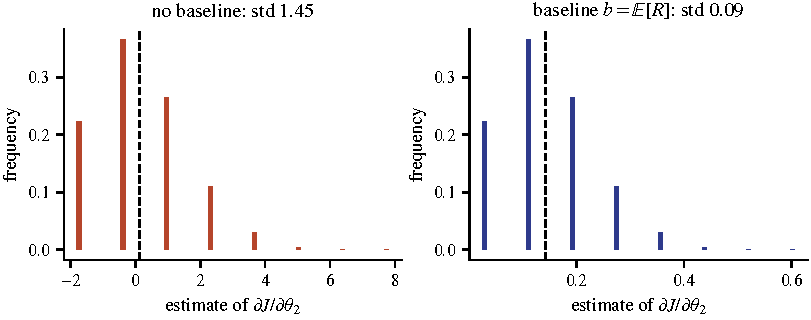
\includegraphics[width=0.86\linewidth]{figures/n15_reinforce.pdf}
\caption{Distribution of $20\,000$ REINFORCE estimates of $\partial J/\partial\theta_2$ for a softmax policy over five
locations ($\vect{\theta} = (0.4, 0, -0.2, 0.1, 0.3)$, the object at location 2, reward $10 + \ind{\text{location 2}}$),
each averaged over $M = 8$ episodes. Dashed line: the exact gradient, $0.143$. The standard deviation drops from $1.45$ to
$0.09$ with the baseline $b = \E[R]$.}
\label{fig:reinforce}
\end{figure}

\begin{algorithm}[htbp]
\caption{REINFORCE with a baseline for a recurrent attention model}\label{alg:reinforce}
\begin{algorithmic}[1]
\Require image $\x$ and label $y^*$; policy and classifier with parameters $\theta$; baseline $b_\psi(\hv)$; $M$ episodes of
  $T$ glimpses; learning rates
\Function{RAMUpdate}{$\x, y^*$}
  \For{$m = 1, \dots, M$}
    \State $\hv_0 \gets \vect{0}$; \ $\vect{l}_0 \gets$ initial location
    \For{$t = 1, \dots, T$}
      \State $\vect{g}_t \gets$ glimpse network on the patches around $\vect{l}_{t-1}$; \ $\hv_t \gets f_h(\hv_{t-1}, \vect{g}_t)$
      \State $\vect{l}_t \sim \Normal(f_l(\hv_t), \sigma^2 I)$ \Comment{sampled: no gradient through this step}
    \EndFor
    \State $R^{(m)} \gets \ind{\argmax f_a(\hv_T) = y^*}$ \Comment{reward of the episode}
  \EndFor
  \State $\gv_\theta \gets \frac1M\sum_{m}\sum_{t}\big(R^{(m)} - b_\psi(\hv^{(m)}_t)\big)\nabla_\theta\log\Normal\big(\vect{l}^{(m)}_t; f_l(\hv^{(m)}_t), \sigma^2 I\big)$
  \State $\gv_\theta \gets \gv_\theta + \frac1M\sum_m\nabla_\theta\log p_\theta\big(y^* \mid \hv_T^{(m)}\big)$ \Comment{backprop for the classifier}
  \State $\gv_\psi \gets \frac1M\sum_{m,t}\nabla_\psi\big(R^{(m)} - b_\psi(\hv_t^{(m)})\big)^2$ \Comment{fit the baseline}
  \State $\theta \gets \theta + \eta\,\gv_\theta$; \ $\psi \gets \psi - \eta'\gv_\psi$ \Comment{ascent on $J$, descent on the baseline loss}
\EndFunction
\end{algorithmic}
\end{algorithm}

\needspace{6\baselineskip}
\begin{runtime}{recurrent attention model with REINFORCE}
\emph{Time per update}: $MT$ glimpses, each costing the glimpse network on a few small patches of $P$ pixels, $O(Pd_g)$, and
an RNN step, $O(d_h^2 + d_hd_g)$, plus the same again for the backward pass. None of this depends on the image size. \emph{Memory}: $O(MT(d_h + d_g))$ for the episode
states. \emph{Sample efficiency} is the hidden cost: the variance of the estimator means many more updates than for a
model trained by backpropagation alone. \emph{Prediction}: one episode of $T$ glimpses.
\end{runtime}

\subsection{Soft versus hard, and soft attention for images}\label{sec:softhard}

Table~\ref{tab:softhard} compares the two kinds of attention.

\begin{table}[htbp]
\centering\small
\caption{Soft and hard attention.}
\label{tab:softhard}
\begin{tabular}{@{}L{0.24\linewidth}L{0.33\linewidth}L{0.33\linewidth}@{}}
\toprule
& soft (content-based, Section~\ref{sec:soft}) & hard (RAM, this section) \\
\midrule
what is learned & a scoring function & a sampling policy \\
output of the mechanism & weights on all positions & one sampled position \\
gradient & exact, by backpropagation & estimated by REINFORCE (Algorithm~\ref{alg:reinforce}) \\
gradient variance & none & high, reduced by a baseline (Figure~\ref{fig:reinforce}) \\
cost per step & $O(\text{input size})$ & $O(1)$ in the input size \\
memory for backprop & all weights & only the sampled path \\
examples in this note & Algorithm~\ref{alg:attdec}, Show, attend and tell, DRAW & RAM (Algorithm~\ref{alg:reinforce}) \\
\bottomrule
\end{tabular}
\end{table}

The two kinds are not tied to their first applications. Soft content-based attention works on images: in \emph{Show, attend
and tell}~\cite{xu2015} a convnet turns an image into a $14 \times 14$ grid of feature vectors, and an LSTM that writes a
caption attends over the 196 positions at each word, exactly as in \eqref{eq:alpha}--\eqref{eq:context}; the same paper also
trained a stochastic hard version. Conversely, hard attention has been used for sequence-to-sequence tasks: Luo et al.\
trained a model that decides online, by sampling, when to emit an output token, with the REINFORCE estimator of
Section~\ref{sec:reinforce}; it works, but needs careful variance reduction to train stably, as the analysis of that
section leads one to expect~\cite{luo2016}.

\paragraph{DRAW: soft location-based attention for images} The DRAW network of Gregor et al.~\cite{gregor2015} generates
images by repeatedly reading from and writing to a canvas through a differentiable window: an $N \times N$ grid of Gaussian
filters whose centre $(g_X, g_Y)$, stride $\delta$, width $\sigma$ and intensity $\gamma$ the network emits at each step.
Filter $i$ along $x$ is centred at $\mu_X^i = g_X + (i - N/2 - 1/2)\,\delta$; the matrix $F_X \in \R^{N \times A}$ has
row-normalised entries proportional to $\exp\big(-(a - \mu_X^i)^2/(2\sigma^2)\big)$, and similarly $F_Y$. The glimpse of an
image $\X \in \R^{B \times A}$ ($B$ rows, $A$ columns; $F_Y \in \R^{N \times B}$) is the patch $\gamma F_Y\X F_X\T$: a small stride zooms in, a large one sees the whole image
coarsely. Like Graves' window it is location-based and soft, so plain backpropagation trains it.

\section{Self-attention and the transformer}\label{sec:transformer}

The attention of Section~\ref{sec:soft} connects a decoder to an encoder that is still recurrent. Vaswani et
al.~\cite{vaswani2017} showed that attention can also be used \emph{inside} the encoder and the decoder, replacing
recurrence and convolution entirely. The resulting \emph{transformer} became the standard architecture for language, and increasingly for
other data.

\subsection{Generalised dot-product attention}\label{sec:sdpa}

Abstract from the decoder and the encoder. A \emph{query} $\qv \in \R^{d_k}$ is compared with $T_k$ \emph{keys}
$\kv_1, \dots, \kv_{T_k} \in \R^{d_k}$, and the result is a weighted average of $T_k$ \emph{values} $\vv_1, \dots, \vv_{T_k} \in
\R^{d_v}$:
\begin{equation}\label{eq:attvec}
  A(\qv; K, V) = \sum_{j=1}^{T_k}\frac{\exp(\qv\T\kv_j/\sqrt{d_k})}{\sum_{m=1}^{T_k}\exp(\qv\T\kv_m/\sqrt{d_k})}\,\vv_j .
\end{equation}
In Section~\ref{sec:soft} the query was the decoder state and keys and values were both the encoder states; separating
keys from values lets a position be found by one description and deliver another. Note~5, Section~3.3 (modern box),
read \eqref{eq:attvec} as a Nadaraya--Watson smoother with an exponential kernel whose queries, keys and values are learned
(Section~\ref{sec:selfatt}). Stacking $T_q$ queries as the rows of $Q \in \R^{T_q \times d_k}$, and keys and values as the rows of
$K \in \R^{T_k \times d_k}$ and $V \in \R^{T_k \times d_v}$, all queries are answered at once:
\begin{equation}\label{eq:attmat}
  \mathrm{Attention}(Q, K, V) = \softmax\!\Big(\frac{QK\T}{\sqrt{d_k}}\Big)V \in \R^{T_q \times d_v},
\end{equation}
with the softmax taken along each row ($V$ is not the vocabulary here). Two matrix products and a row-wise softmax: exactly the operations that GPUs do best.

\paragraph{Derivation: why divide by $\sqrt{d_k}$} Suppose that at initialisation the components of $\qv$ and $\kv$ are
independent with mean $0$ and variance $1$, as they roughly are when the inputs are layer-normalised and the projections use
a variance-preserving initialisation. Then $\qv\T\kv = \sum_{a=1}^{d_k}q_ak_a$ is a sum of $d_k$ independent terms,
each with mean $\E[q_a]\E[k_a] = 0$ and variance
\[
  \Var(q_ak_a) = \E[q_a^2k_a^2] - (\E[q_ak_a])^2 = \E[q_a^2]\,\E[k_a^2] - 0 = 1 ,
\]
so $\Var(\qv\T\kv) = d_k$ and the scores have standard deviation $\sqrt{d_k}$ (the computation behind Glorot and He
initialisation, Note~12, Section~7). For $d_k = 64$ the scores have standard deviation $8$ and two scores typically differ
by about $11$; the softmax of such scores is nearly one-hot, and by \eqref{eq:gradscore} its gradient nearly
vanishes. Dividing by $\sqrt{d_k}$ restores unit variance whatever the width; in the language of the physics box of
Section~\ref{sec:alignvis}, it sets the temperature to $\sqrt{d_k}$. Figure~\ref{fig:scaling} measures the effect for 32
random keys: without scaling the entropy of the weights collapses as $d_k$ grows and the median Jacobian of the softmax
falls by two orders of magnitude at $d_k = 512$; with scaling both stay constant.

\begin{figure}[htbp]
\centering
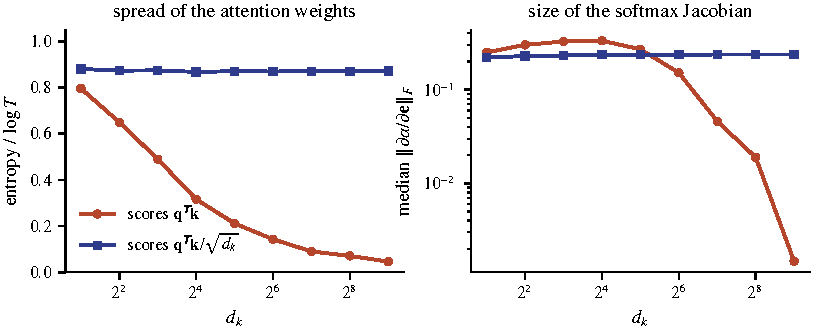
\includegraphics[width=0.86\linewidth]{figures/n15_scaling.pdf}
\caption{Softmax over $T = 32$ keys with standard normal queries and keys, over 2000 draws. Left: mean entropy of the
weights divided by its maximum $\log T$. Right: median Frobenius norm of the Jacobian $\diag(\valpha) - \valpha\valpha\T$.
With unscaled scores the entropy ratio falls to $0.14$ at $d_k = 64$ and to $0.05$ at $d_k = 512$, and the median Jacobian
to $0.0015$ at $d_k = 512$; with scaled scores both stay near $0.87$ and $0.24$.}
\label{fig:scaling}
\end{figure}

\subsection{Self-attention and masks}\label{sec:selfatt}

In \emph{self-attention} a sequence attends to itself. The rows of $X \in \R^{T \times d}$ are the representations of
the $T$ positions, and queries, keys and values are three learned linear maps of the same rows:
\begin{equation}\label{eq:selfatt}
  Q = XW_Q, \quad K = XW_K, \quad V = XW_V, \qquad \text{output} = \softmax\!\Big(\frac{QK\T}{\sqrt{d_k}} + M\Big)V ,
\end{equation}
with $W_Q, W_K \in \R^{d \times d_k}$, $W_V \in \R^{d \times d_v}$, and a \emph{mask} $M \in \{0, -\infty\}^{T \times T}$
added to the scores. An entry $-\infty$ gives the weight $e^{-\infty} = 0$, so it forbids position $i$ to read position
$j$. Two masks are common:
\begin{itemize}
\item the \emph{causal} mask, $M_{ij} = -\infty$ for $j > i$, lets every position see only itself and the past. It is what
  makes a transformer a valid autoregressive model, $p(y_i \mid y_{<i})$, as in \eqref{eq:seq2seq};
\item the \emph{padding} mask hides the filler positions added to make the sequences of a mini-batch equally long.
\end{itemize}
In a decoder the input sequence is the target shifted right by one, $(\texttt{<bos>}, y_1, \dots, y_{T'-1})$, so
position $i$ holds $y_{i-1}$ and, with the causal mask, its output depends on $y_{<i}$ only; that output predicts $y_i$.

\begin{worked}{6. Self-attention on three tokens}
Three tokens with $d = d_k = d_v = 2$ have the rows $\x_1 = (1, 0)$, $\x_2 = (0, 1)$, $\x_3 = (1, 1)$ and
\[
  W_Q = \begin{pmatrix} 1 & 1 \\ 0 & 1 \end{pmatrix}, \quad W_K = \begin{pmatrix} 1 & 0 \\ 1 & 1 \end{pmatrix}, \quad
  W_V = \begin{pmatrix} 1 & 0 \\ 0 & 2 \end{pmatrix}, \quad \text{so that}
\]
\[
  Q = \begin{pmatrix} 1 & 1 \\ 0 & 1 \\ 1 & 2 \end{pmatrix}, \quad
  K = \begin{pmatrix} 1 & 0 \\ 1 & 1 \\ 2 & 1 \end{pmatrix}, \quad
  V = \begin{pmatrix} 1 & 0 \\ 0 & 2 \\ 1 & 2 \end{pmatrix}.
\]
\emph{Scores.} $QK\T$ has the rows $(1, 2, 3)$, $(0, 1, 1)$, $(1, 3, 4)$; divided by $\sqrt2$ they become $(0.707, 1.414,
2.121)$, $(0, 0.707, 0.707)$, $(0.707, 2.121, 2.828)$.
\emph{Weights.} Row 1 has the scores of Worked example~1, so its weights are the scaled-dot weights found there; rows 2
and 3 follow in the same way:
\[
  A = \begin{pmatrix} 0.140 & 0.284 & 0.576 \\ 0.198 & 0.401 & 0.401 \\ 0.074 & 0.306 & 0.620 \end{pmatrix}, \qquad
  AV = \begin{pmatrix} 0.716 & 1.720 \\ 0.599 & 1.604 \\ 0.694 & 1.851 \end{pmatrix}.
\]
Token~2 attends equally to tokens 2 and~3 because their keys give it the same score.
\emph{Causal mask.} Setting the scores above the diagonal to $-\infty$ leaves row 1 with the single weight $1$ (output
$\vv_1 = (1, 0)$), row 2 with $\softmax(0, 0.707) = (0.330, 0.670)$ (output $(0.330, 1.340)$), and row 3 unchanged. The first
token now knows nothing about its successors, which is what a model that predicts the next token requires.
\end{worked}

\begin{physics}{permutation symmetry and the need for positions}
Let $P$ be a $T \times T$ permutation matrix, so that $PX$ lists the same tokens in another order. Then $(PX)W_Q = PQ$,
similarly for $K$ and $V$, and
\[
\begin{aligned}
  \softmax\big(PQ(PK)\T/\sqrt{d_k}\big)PV &= \softmax\big(P\,QK\T P\T/\sqrt{d_k}\big)PV \\
  &= P\,\softmax\big(QK\T/\sqrt{d_k}\big)P\T P V = P\,\big(\text{output}\big),
\end{aligned}
\]
because a row-wise softmax commutes with permuting rows and columns, and $P\T P = I$. Self-attention without a mask is
\emph{permutation equivariant}: it treats its input as a set of interacting particles, much like a system of identical
particles with pairwise (though not necessarily reciprocal) interactions, whose dynamics does not care how the particles
are labelled. For particles in a
jet, atoms in a molecule or galaxies in a survey this is the right symmetry, and transformers without positional
information are natural models for them. For language (as for Note~1's bag of words) it is wrong: ``dog bites man'' and ``man bites dog'' would get the
same representations, permuted. The order must be supplied explicitly (Section~\ref{sec:posenc}). A causal mask also breaks
the symmetry, because it singles out an order.
\end{physics}

\subsection{Multi-head attention}\label{sec:mha}

One attention operation produces, at each position, one weighted average: one way of choosing what to read. Multi-head
attention runs $h$ attention operations in parallel, each in its own lower-dimensional subspace, and concatenates the
results:
\begin{equation}\label{eq:mha}
  \mathrm{head}_r = \mathrm{Attention}\big(XW_Q^{(r)}, XW_K^{(r)}, XW_V^{(r)}\big), \qquad
  \mathrm{MHA}(X) = [\mathrm{head}_1, \dots, \mathrm{head}_h]\,W_O ,
\end{equation}
with $W_Q^{(r)}, W_K^{(r)}, W_V^{(r)} \in \R^{d \times d/h}$ and $W_O \in \R^{d \times d}$. One head may track the previous
token, another the subject of the verb, a third the matching bracket. With $d_k = d_v = d/h$ the number of parameters,
$4d^2$ plus $4d$ biases, and the number of multiply--adds do not depend on $h$ (only the $hT^2$ softmax evaluations and
stored weights grow with $h$): the heads split the width, they do not multiply it.

\begin{algorithm}[htbp]
\caption{Multi-head (masked) self-attention, forward pass}\label{alg:mha}
\begin{algorithmic}[1]
\Require $X \in \R^{T \times d}$; $h$ heads with $d_k = d/h$; $W_Q, W_K, W_V, W_O \in \R^{d \times d}$ (the head blocks side by
  side) and biases; mask $M$ (causal, padding, or none)
\Function{MultiHeadAttention}{$X$; $M$}
  \State $Q \gets XW_Q$, \ $K \gets XW_K$, \ $V \gets XW_V$ \Comment{three $T \times d$ products, $O(Td^2)$ each}
  \For{$r = 1, \dots, h$} \Comment{all heads in parallel in practice}
    \State $Q_r, K_r, V_r \gets$ columns $(r - 1)d_k + 1, \dots, rd_k$ of $Q, K, V$
    \State $S_r \gets Q_rK_r\T/\sqrt{d_k} + M$ \Comment{$T \times T$ scores, $O(T^2d_k)$}
    \State $A_r \gets$ row-wise softmax of $S_r$ (subtract each row's maximum first)
    \State $H_r \gets A_rV_r$ \Comment{$O(T^2d_k)$}
  \EndFor
  \State \Return $[H_1, \dots, H_h]\,W_O$ \Comment{$O(Td^2)$}
\EndFunction
\end{algorithmic}
\end{algorithm}

\needspace{10\baselineskip}
\begin{runtime}{multi-head self-attention}
\emph{Time}: $4Td^2$ multiply--adds for the four projections and $2T^2d$ for scores and weighted sums (summed over the
$h$ heads, $h \cdot 2T^2d_k = 2T^2d$), so $O(Td^2 + T^2d)$ per layer and sequence; the second term dominates once $T > 2d$
when only attention is counted. \emph{Memory}: $O(Td)$ for the activations and $O(hT^2)$ for the attention weights, which a
standard implementation stores for the backward pass. \emph{Parallelism}: unlike an RNN, all $T$ positions are processed at
once; the sequential depth of a layer is $O(1)$, and the path between any two positions has length one. For comparison, a
recurrent layer costs $O(Td^2)$ but needs $T$ sequential steps, and the path between positions $i$ and $j$ has length
$|i - j|$ (Note~14, Section~2). \emph{Backward}: about twice the forward.
\end{runtime}

\subsection{Three kinds of attention in the transformer}\label{sec:threekinds}

The encoder--decoder transformer of Vaswani et al.\ uses attention in three places.
\begin{enumerate}
\item \emph{Encoder self-attention}: $Q$, $K$ and $V$ all come from the encoder's representation of the source sentence,
  with only a padding mask. Every source position can read every other one; this replaces the bidirectional RNN.
\item \emph{Masked decoder self-attention}: $Q$, $K$ and $V$ come from the decoder's representation of the target prefix,
  with a causal mask. This replaces the decoder RNN. During training, with teacher forcing (Note~14, Section~7), all target
  positions are computed in parallel in one pass, the shifted input and the mask guaranteeing that the output at position
  $i$, which predicts $y_i$, never depends on $y_i, y_{i+1}, \dots$
\item \emph{Encoder--decoder (cross-) attention}: queries from the decoder, keys and values from the final encoder output.
  This is the attention of Section~\ref{sec:soft}, with a scaled dot-product score instead of the additive one.
\end{enumerate}

\subsection{Positional information}\label{sec:posenc}

Because self-attention is permutation equivariant, the transformer adds a vector $\pv_t \in \R^d$ that depends only on the
position $t$ to the embedding of the token at position $t$. The original choice is a set of sinusoids of geometrically
spaced frequencies,
\begin{equation}\label{eq:posenc}
  p_{t,2i} = \sin(\omega_it), \qquad p_{t,2i+1} = \cos(\omega_it), \qquad \omega_i = 10\,000^{-2i/d}, \quad i = 0, \dots, d/2 - 1 ,
\end{equation}
with wavelengths from $2\pi$ up to about $2\pi \cdot 10^4$ positions (Figure~\ref{fig:posenc}). \emph{Learned} position
embeddings, one trainable vector per position, work about as well in translation~\cite{vaswani2017} but cannot be used beyond
the longest training position.

\paragraph{Derivation: relative positions are linear} For one frequency $\omega$, the addition theorems give
\[
  \begin{pmatrix} \sin\omega(t + k) \\ \cos\omega(t + k) \end{pmatrix}
  = \begin{pmatrix} \cos\omega k & \sin\omega k \\ -\sin\omega k & \cos\omega k \end{pmatrix}
  \begin{pmatrix} \sin\omega t \\ \cos\omega t \end{pmatrix} ,
\]
so $\pv_{t+k} = R_k\pv_t$ with a block-diagonal rotation $R_k$ that depends on the offset $k$ but not on $t$. A linear map
can therefore express ``the position $k$ steps back'', and the dot product
\[
  \pv_t\T\pv_{t+k} = \sum_i\big[\sin\omega_it\,\sin\omega_i(t + k) + \cos\omega_it\,\cos\omega_i(t + k)\big] = \sum_i\cos\omega_ik
\]
depends on the offset only, as the right panel of Figure~\ref{fig:posenc} confirms (the three curves agree to $10^{-14}$).

\begin{figure}[htbp]
\centering
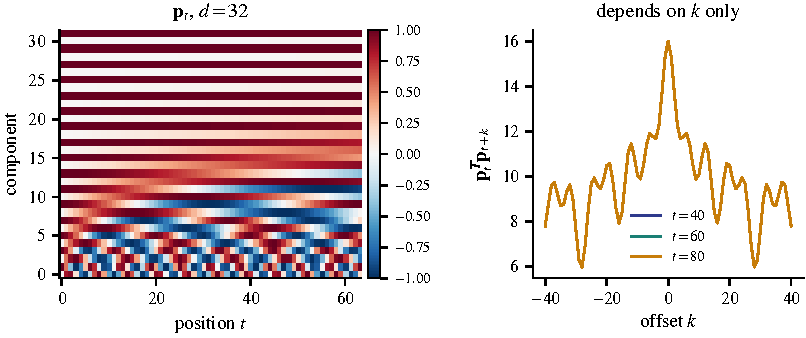
\includegraphics[width=0.86\linewidth]{figures/n15_posenc.pdf}
\caption{Left: the sinusoidal encodings \eqref{eq:posenc} for $d = 32$ and the first 64 positions; low components oscillate
fast, high ones slowly, like the digits of a continuous binary counter. Right: $\pv_t\T\pv_{t+k}$ as a function of the
offset $k$ for three starting positions $t$; the curves coincide, with maximum $d/2 = 16$ at $k = 0$.}
\label{fig:posenc}
\end{figure}

\begin{modern}{rotary position embeddings}
Instead of adding positions to the input, \emph{rotary position embeddings} (RoPE)~\cite{su2024} rotate each pair of
components of the query at position $m$ by the angle $m\omega_i$ and the key at position $n$ by $n\omega_i$, with the
frequencies of \eqref{eq:posenc}. Rotations are orthogonal, so $(R_m\qv)\T(R_n\kv) = \qv\T R_m\T R_n\kv = \qv\T R_{n-m}\kv$:
the score depends on the content and on the \emph{relative} position $n - m$ only, in every layer. Many current open
language models use RoPE, and several methods that extend their context length work by rescaling its frequencies.
\end{modern}

\subsection{The block and the full model}\label{sec:block}

A transformer layer combines self-attention, which mixes information \emph{between} positions, with a position-wise MLP,
which processes each position separately with the same weights (Note~11, Section~4: one hidden layer of width $d_{\mathrm{ff}}$,
usually $4d$, with ReLU or GELU). Each of the two sublayers is wrapped in a residual connection and a layer normalisation,
whose purpose and derivation are those of Note~12, Sections~10.2 and~10.3. In the \emph{pre-normalisation} form, whose
stability advantage over the original post-normalisation is discussed in Note~12, Section~10.3 (modern box),
\begin{equation}\label{eq:block}
  X \gets X + \mathrm{MHA}\big(\LN(X)\big), \qquad X \gets X + \MLP\big(\LN(X)\big) .
\end{equation}
The full model of Vaswani et al.\ adds positional
encodings to token embeddings (scaled by $\sqrt{d}$), stacks $N = 6$ encoder layers and $N = 6$ decoder layers (each decoder
layer with masked self-attention, cross-attention and an MLP), and ends with a linear map to the vocabulary and a softmax that
shares its weight matrix with the embeddings. The base model ($d = 512$, $h = 8$, $d_{\mathrm{ff}} = 2048$) trained for about twelve hours on eight GPUs and already
outperformed all previously published models on English--German translation, and a larger version set a new single-model
record on English--French~\cite{vaswani2017}; training was much faster than for recurrent models because no step waits for
the previous one.

\begin{algorithm}[htbp]
\caption{Transformer layer (pre-normalisation), encoder or decoder}\label{alg:block}
\begin{algorithmic}[1]
\Require $X \in \R^{T \times d}$; for a decoder layer also the encoder output $Z \in \R^{T_{\mathrm{src}} \times d}$; masks
\Function{TransformerLayer}{$X$; $Z$}
  \State $X \gets X + \Call{MultiHeadAttention}{\LN_1(X); M}$ \Comment{Algorithm~\ref{alg:mha}; $M$ causal in a decoder}
  \If{decoder of an encoder--decoder model}
    \State $X \gets X + \textsc{CrossAttention}\big(\LN_2(X), Z\big)$ \Comment{queries from $X$, keys and values from $Z$}
  \EndIf
  \State $X \gets X + \max(0, \LN_3(X)W_1 + \onev\vect{b}_1\T)\,W_2 + \onev\vect{b}_2\T$ \Comment{position-wise MLP, $W_1 \in \R^{d \times d_{\mathrm{ff}}}$}
  \State \Return $X$
\EndFunction
\end{algorithmic}
\end{algorithm}

\begin{runtime}{one transformer layer}
\emph{Time}: $4Td^2$ for the attention projections, $2T^2d$ for scores and mixing, and $2Tdd_{\mathrm{ff}} = 8Td^2$ for the
MLP with $d_{\mathrm{ff}} = 4d$: in total $12Td^2 + 2T^2d$ multiply--adds per layer. A decoder layer adds
$2Td^2 + 2T_{\mathrm{src}}d^2$ for the cross-attention projections (the latter once per source sentence) and
$2TT_{\mathrm{src}}d$ for its scores and mixing.
\emph{Memory}: $12d^2 + O(d)$ parameters per layer (16$d^2$ with cross-attention); activations $O(Td + Td_{\mathrm{ff}})$
and attention weights $O(hT^2)$ per layer and sequence for the backward pass. \emph{A model of $L$ layers}: $L$ times
this; training costs about three forward passes per example.
\end{runtime}

\begin{worked}{7. Shapes and parameters of the base transformer}
Take $d = 512$, $h = 8$ (so $d_k = 64$), $d_{\mathrm{ff}} = 2048$ and a source sentence of $T = 20$ tokens.
\emph{Shapes in one encoder layer:} $X$ is $20 \times 512$; $Q, K, V$ are $20 \times 512$, split into eight $20 \times 64$
blocks; each head has a $20 \times 20$ weight matrix and a $20 \times 64$ output; the concatenation and $W_O$ return
$20 \times 512$; the MLP goes through $20 \times 2048$ and back to $20 \times 512$. Every layer maps $T \times d$ to
$T \times d$, which is why layers can be stacked and the residual additions are possible.
\emph{Parameters:} attention $4(512^2 + 512) = 1\,050\,624$; MLP $512 \cdot 2048 + 2048 + 2048 \cdot 512 + 512 =
2\,099\,712$; two layer norms $2 \cdot 2 \cdot 512 = 2048$; so an encoder layer has $3\,152\,384$ parameters, two thirds of them in the MLP, as for GPT-2 in Note~11, Section~4.2;
a decoder layer adds cross-attention and a
third layer norm, $4\,204\,032$. Six of each give $44.1$ million, and a shared embedding table for a vocabulary of about
$37\,000$ tokens adds $37\,000 \times 512 = 18.9$ million, about $63$ million in all; Vaswani et al.\ report $65$ million for
the base model.
\emph{Cost:} for $T = 20$ the attention scores are a negligible $2T^2d = 4.1 \times 10^5$ multiply--adds per layer against
$12Td^2 = 6.3 \times 10^7$; for $T = 3072 = 6d$ the two are equal.
\end{worked}


\begin{physics}{tokens as interacting particles}
Read the rows $\x_1, \dots, \x_T$ of $X$ as the positions of $T$ particles in $\R^d$ and the layer index as time. For a
single head with $d_v = d$ and ignoring the layer norm, one self-attention sublayer with its residual connection is
\[
  \x_i \gets \x_i + \sum_j \frac{e^{\beta\,\x_i\T B\,\x_j}}{\sum_m e^{\beta\,\x_i\T B\,\x_m}}\, U\x_j ,
  \qquad B = W_QW_K\T, \quad U = (W_VW_O)\T, \quad \beta = 1/\sqrt{d_k}
\]
(with $h$ heads the update is a sum of $h$ such terms). It is an explicit Euler step of a system in which each particle is
displaced by a linear map $U$ of a weighted average of all particles (itself included), with weights set by a pairwise
interaction $B$; with layer normalisation the particles move on a sphere. When $T$ is large the sum is an average over the empirical distribution of particles: a
\emph{mean-field} dynamics, of the same form as the Vlasov-type equations of plasma physics or models of flocking.
Geshkovski et al.\ analyse transformers in exactly this way and find that, in simplified settings, the particles tend to
form clusters as depth grows~\cite{geshkovski2023}. A related reading identifies the attention update with one step of a
modern Hopfield network, which retrieves the stored pattern closest to a query~\cite{ramsauer2021}.
\end{physics}

\section{Decoder-only models and efficient attention}\label{sec:modern}

\subsection{Decoder-only language models}\label{sec:decoderonly}

Drop the encoder and the cross-attention, keep the masked decoder: a stack of causal self-attention layers trained to
predict the next token is a language model, $p(y_1, \dots, y_T) = \prod_i p(y_i \mid y_{<i})$, of the kind that Note~14,
Sections~1 and~2, built from RNNs. The GPT models~\cite{radford2019,brown2020} are of this type, and so are almost all current large language models;
a translation, a question or a program is presented as a prefix (the \emph{prompt}) and the answer generated as its
continuation. Encoder-only models such as BERT~\cite{devlin2019} use unmasked self-attention and are trained to recover
input tokens that were hidden by a special token (a different use of the word \emph{mask}). Training computes the loss
at all $T$ positions in parallel (Section~\ref{sec:threekinds}), whereas an RNN must compute its states one after the
other, and it needs no labels, so very large text collections can be used. Text is generated one token at a time, by
greedy choice, beam search or sampling with a temperature or a nucleus (Note~14, Section~8); the next subsection makes
this generation efficient.

\subsection{The key--value cache}\label{sec:kvcache}

At generation step $t$ the new token must attend to all $t$ previous positions in every layer. Their keys and values do not
change when a token is appended --- the causal mask guarantees that earlier positions never see later ones --- so they are
computed once and stored: the \emph{key--value (KV) cache}. Each step then only computes the query, key and value of the
\emph{new} position. In Algorithm~\ref{alg:kv} the prefill stops one token short, so that the loop handles $y_P$ and
every position enters the cache exactly once.

\begin{algorithm}[htbp]
\caption{Autoregressive generation with a key--value cache (decoder-only model)}\label{alg:kv}
\begin{algorithmic}[1]
\Require prompt $y_1, \dots, y_P$; $L$ layers; output (unembedding) matrix $W_U \in \R^{V \times d}$; number of new tokens
  $N$; a decoding rule (greedy, beam, sampling)
\Function{Generate}{$y_{1:P}$}
  \State run $y_1, \dots, y_{P-1}$ through all layers with the causal mask; keep $K^{(l)}, V^{(l)} \in \R^{(P-1) \times d}$
    \Comment{prefill}
  \For{$t = P + 1, \dots, P + N$}
    \State $\x \gets$ embedding of $y_{t-1}$ plus position $t - 1$ \Comment{one row}
    \For{$l = 1, \dots, L$}
      \State $\qv, \kv, \vv \gets$ projections of $\LN(\x)$; \ append $\kv$ to $K^{(l)}$ and $\vv$ to $V^{(l)}$ \Comment{$O(d^2)$}
      \State $\x \gets \x + [\softmax(K^{(l)}_r\qv_r/\sqrt{d_k})\T V^{(l)}_r]_{r = 1, \dots, h}\,W_O$ \Comment{$O(td)$ over the cache}
      \State $\x \gets \x + \MLP(\LN(\x))$ \Comment{$O(d^2)$}
    \EndFor
    \State $y_t \gets$ decoding rule applied to $\softmax(W_U\LN(\x))$ \Comment{$O(dV)$}
  \EndFor
  \State \Return $y_{P+1:P+N}$
\EndFunction
\end{algorithmic}
\end{algorithm}

\begin{runtime}{generation with and without a KV cache}
\emph{With the cache}, step $t$ costs $O\big(L(d^2 + td) + dV\big)$: the projections and MLP of one position and attention over
$t$ cached keys. Generating $N$ tokens after a prompt of $P$ costs $O\big(L(Pd^2 + P^2d)\big)$ for the prefill plus
$O\big(L(Nd^2 + N(P + N)d) + NdV\big)$. \emph{Without the cache}, every step reruns the whole prefix, $O(L(td^2 + t^2d))$,
and $N$ steps cost $O\big(L(N(P + N)d^2 + N(P + N)^2d)\big)$. \emph{Memory}: the cache holds $2LTd$ numbers
for $T$ cached tokens, per sequence; at long contexts it, not the weights, limits the batch size. Each step reads the
whole cache and all weights while doing little arithmetic per number read: generation is limited by memory bandwidth.
\end{runtime}

\begin{worked}{8. How large is the cache}
A hypothetical model has $L = 32$ layers of width $d = 4096$ with $h = 32$ heads, stored in 16-bit numbers (two bytes). Per
token the cache holds a key and a value of size $d$ in every layer: $2 \cdot 32 \cdot 4096 \cdot 2 = 524\,288$ bytes, half a
mebibyte. A context of $T = 4096$ tokens needs $2^{19} \cdot 2^{12} = 2^{31}$ bytes $= 2$~GiB per sequence, and a batch of 16
such sequences $32$~GiB. \emph{Multi-query attention}~\cite{shazeer2019} lets all 32 query heads share a single key and value
head, which divides the cache by 32 (64~MiB); \emph{grouped-query attention}~\cite{ainslie2023} shares one key--value head
among each group of query heads, for example 8 groups of 4, which divides it by 4 (0.5~GiB) with less loss of quality.
\end{worked}

\subsection{IO-aware exact attention}\label{sec:flash}

A standard implementation of \eqref{eq:attmat} writes the $T \times T$ score matrix to the GPU's main memory, reads it back
for the softmax, writes the weights, and reads them again for the product with $V$. For long sequences this traffic, not the
arithmetic, dominates the time, and the $O(T^2)$ memory limits $T$. FlashAttention~\cite{dao2022} computes exactly the same
result without ever forming the full matrix: it loads blocks of $Q$, $K$ and $V$ into the small, fast on-chip memory and
combines the partial results with an \emph{online softmax}.

\paragraph{Derivation: merging two softmax blocks} Split the scores of one query into two blocks. For each block keep its
maximum $m$, the sum $Z = \sum_j e^{s_j - m}$ (a partial partition function) and the unnormalised output $\vect{o} = \sum_j e^{s_j - m}\vv_j$. With
$m = \max(m_1, m_2)$, rescaling each block to the common maximum gives
\begin{equation}\label{eq:online}
  Z = e^{m_1 - m}Z_1 + e^{m_2 - m}Z_2, \qquad \vect{o} = e^{m_1 - m}\vect{o}_1 + e^{m_2 - m}\vect{o}_2, \qquad
  \text{output} = \vect{o}/Z ,
\end{equation}
exactly the full softmax average, because $e^{m_b - m}e^{s_j - m_b} = e^{s_j - m}$. The blocks can therefore be processed one
after the other, keeping only $m$, $Z$ and $\vect{o}$ --- the log-sum-exp trick of Note~5, Section~3.3, made incremental.

\begin{worked}{9. Online softmax in two blocks}
One query has scores $\vect{s} = (1, 3, 2 \mid 5, 0)$ for values $(2, -1, 0 \mid 1, 4)$ (scalars for simplicity).
\emph{Block 1:} $m_1 = 3$, $Z_1 = e^{-2} + e^0 + e^{-1} = 0.1353 + 1 + 0.3679 = 1.5032$,
$o_1 = 2e^{-2} - 1 + 0 = -0.7293$.
\emph{Block 2 arrives:} $m = 5$, so the old quantities are multiplied by $e^{3 - 5} = 0.1353$:
$Z = 0.2034 + e^0 + e^{-5} = 1.2102$ and $o = -0.0987 + 1 + 4e^{-5} = 0.9282$.
\emph{Output:} $0.9282/1.2102 = 0.7670$, identical to the softmax average computed in one go.
\end{worked}

\begin{algorithm}[htbp]
\caption{Tiled attention with an online softmax (forward pass, one block of queries)}\label{alg:flash}
\begin{algorithmic}[1]
\Require a block $Q_b$ of $B_q$ queries; keys and values in blocks $K_c, V_c$ of $B_k$ rows, $c = 1, \dots, \lceil T/B_k\rceil$
\Function{TiledAttention}{$Q_b$}
  \State $\vect{m} \gets -\infty$, \ $\zv \gets \vect{0}$ (one entry per query), \ $O \gets 0 \in \R^{B_q \times d_v}$
  \For{$c = 1, \dots, \lceil T/B_k\rceil$} \Comment{with a causal mask, skip blocks entirely in the future}
    \State load $K_c, V_c$ into fast memory; \ $S \gets Q_bK_c\T/\sqrt{d_k}$ (plus mask) \Comment{$B_q \times B_k$, never written out}
    \State $\vect{m}' \gets \max(\vect{m}, \text{row maxima of } S)$; \ $P \gets \exp(S - \vect{m}')$ row-wise
    \State $\zv \gets e^{\vect{m} - \vect{m}'} \odot \zv + \text{row sums of } P$; \
      $O \gets \diag(e^{\vect{m} - \vect{m}'})\,O + PV_c$; \ $\vect{m} \gets \vect{m}'$
  \EndFor
  \State \Return $\diag(\zv)^{-1}O$ and $\log\zv + \vect{m}$ \Comment{the latter lets the backward pass recompute $P$}
\EndFunction
\end{algorithmic}
\end{algorithm}

\needspace{6\baselineskip}
\begin{runtime}{tiled (IO-aware) attention}
\emph{Arithmetic}: the same $O(T^2d)$ multiply--adds as the standard algorithm, plus $O(T^2d_v/B_k)$ operations to rescale
the running outputs; the result is
exact, not an approximation. \emph{Extra memory}: $O(T)$ for $\vect{m}$ and $\zv$ instead of $O(T^2)$ for the weights.
\emph{Memory traffic}: with fast memory of size $S_{\mathrm{M}}$ the number of reads and writes of main memory is
$O(T^2d^2/S_{\mathrm{M}})$ against $O(Td + T^2)$ for the standard algorithm~\cite{dao2022}, a large saving for typical $d$ and
$S_{\mathrm{M}}$. \emph{Backward}: the weights are recomputed block by block from $Q$, $K$ and the stored $\log\zv +
\vect{m}$ instead of being read from memory --- more arithmetic, less traffic, and faster overall.
\end{runtime}

\begin{modern}{attention beyond text}
The same block now processes most kinds of data once they are cut into tokens. The \emph{vision transformer} cuts an image
into $16 \times 16$ patches (a strided convolution, Note~13, Section~7) and runs a transformer encoder on the
sequence of patches~\cite{dosovitskiy2021}. CLIP trains an image encoder and a text encoder so that matching image--caption
pairs have large dot products, over hundreds of millions of pairs~\cite{radford2021}. In
\emph{mixture-of-experts} layers the single MLP of each block is replaced by many expert MLPs, and a small router sends each
token to the top one or two~\cite{shazeer2017,fedus2022}: the number of parameters grows while the cost per token stays
nearly constant. And the quadratic cost of attention has revived recurrence: state-space models such as S4 and Mamba process
long sequences in linear time with a learned linear recurrence~\cite{gu2022,gu2023} (Note~14, Section~11).
\end{modern}

\begin{physics}{transformers on physics data}
In particle physics a jet is a variable-size \emph{set} of particles, each with momentum, charge and identity. The Particle
Transformer~\cite{qu2022} treats the particles as tokens without positional encodings --- so that it is permutation
equivariant, as the physics demands --- and adds to the attention scores a bias computed from physically motivated pairwise
features such as the angular distance and invariant mass of each pair of particles; it improved jet tagging over earlier
graph networks on a large simulated data set. In structural biology the attention-based network AlphaFold~2 predicts protein
structures from sequences with high accuracy~\cite{jumper2021}. 
\end{physics}

\section{A first look inside a transformer}\label{sec:inside}

\emph{Mechanistic interpretability} tries to find out \emph{how} a trained network computes its predictions: which
components carry which information, and which of them are actually used. This section introduces the vocabulary and the
basic experimental tools, which the course project (weeks 7--14) applies to small models.

\subsection{The residual stream}\label{sec:stream}

Write the pre-normalisation model \eqref{eq:block} for one position $i$ and number all sublayers --- every attention layer
and every MLP --- as components $c = 1, \dots, 2L$. Each component reads the current vector $\x_i$, through a layer norm,
and \emph{adds} its output to it. Unrolling the additions,
\begin{equation}\label{eq:stream}
  \x_i^{\mathrm{final}} = \x_i^{(0)} + \sum_{c=1}^{2L}\vect{o}_i^{(c)}, \qquad
  \text{logits}_i = W_U\,\LN\big(\x_i^{\mathrm{final}}\big),
\end{equation}
where $\x_i^{(0)}$ is the token and position embedding and $\vect{o}_i^{(c)}$ the output of component $c$ at position $i$. The
vector $\x_i$ is called the \emph{residual stream}: a shared $d$-dimensional channel from which every component reads and to
which it writes, and from which the unembedding $W_U$ reads the prediction at the end (Figure~\ref{fig:stream}). An
attention layer is the only component that moves information between positions; MLPs act on each position separately.

\begin{figure}[htbp]
\centering
\begin{tikzpicture}[x=1cm,y=1cm,font=\small,
  comp/.style={draw=indigo,fill=indigo!6,rounded corners=2pt,minimum width=2.6cm,minimum height=0.5cm},
  mlp/.style={draw=teal,fill=teal!8,rounded corners=2pt,minimum width=2.6cm,minimum height=0.5cm}]
  \draw[line width=2.2pt,color=amber!70] (0,0) -- (0,5.0);
  \draw[-{Latex[length=2mm]},line width=1pt,color=amber] (0,4.8) -- (0,5.3);
  \node[anchor=north] at (0,-0.05) {embedding $\x^{(0)}$};
  \node[anchor=south] at (0,5.3) {unembedding $W_U\,\LN(\cdot)$ $\to$ logits};
  \foreach \y/\lab/\sty in {0.35/{attention, layer 1}/comp, 1.45/{MLP, layer 1}/mlp, 2.55/{attention, layer 2}/comp, 3.65/{MLP, layer 2}/mlp} {
    \node[\sty] (b) at (3.0,\y+0.4) {\lab};
    \draw[-{Latex[length=1.5mm]}] (0,\y) -- (1.2,\y) |- (b.west);
    \draw[-{Latex[length=1.5mm]}] (b.east) -- ++(0.35,0) |- (0.16,\y+0.85);
    \node[circle,draw,fill=white,inner sep=0pt,minimum size=0.3cm] at (0,\y+0.85) {$+$};
  }
  \node[font=\scriptsize,color=mute,align=left,anchor=west] at (5.0,0.75) {reads $\LN(\x)$ at all positions,\\writes a mix of them};
  \node[font=\scriptsize,color=mute,align=left,anchor=west] at (5.0,1.85) {reads and writes\\at one position};
  \node[font=\scriptsize,color=mute,anchor=east] at (-0.25,2.5) {residual stream $\x_i$};
\end{tikzpicture}
\caption{The residual-stream view of a two-layer transformer at one position. Every component reads the stream (through a
layer norm) and adds its output back; the final stream is the embedding plus the sum of all outputs.}
\label{fig:stream}
\end{figure}

\paragraph{Heads as two circuits} Ignoring the layer norm, an attention head $r$ writes $\sum_j A^{(r)}_{ij}U^{(r)}\x_j$ to
position $i$, where $W_O^{(r)} \in \R^{d_k \times d}$ is the block of rows of $W_O$ that multiplies the output of head $r$
(so $[H_1, \dots, H_h]W_O = \sum_r H_rW_O^{(r)}$), $U^{(r)} = (W_V^{(r)}W_O^{(r)})\T \in \R^{d \times d}$, and
$A^{(r)}_{ij} \propto \exp(\x_i\T B^{(r)}\x_j/\sqrt{d_k})$, $B^{(r)} = W_Q^{(r)}W_K^{(r)\mathsf{T}}$. Two low-rank matrices thus
describe a head: the \emph{QK circuit} $B^{(r)}$ decides \emph{where} to read, and the \emph{OV circuit} $U^{(r)}$ decides
\emph{what} is written once the position is chosen~\cite{elhage2021}. A head can attend strongly to a token and write almost
nothing, if $U^{(r)}$ is small in the relevant directions.

\paragraph{Direct logit attribution} Freeze the scale factor of the final layer norm at its value on a given input. Then the
logits in \eqref{eq:stream} are a \emph{sum} of contributions, one per component, plus the embedding. For two tokens $a$ and $b$ the \emph{logit difference} splits as
\[
  \text{logit}_a - \text{logit}_b \approx \sum_c \frac{(\uv_a - \uv_b)\T\vect{o}^{(c)}}{\sigma} + (\text{embedding term}),
\]
with $\uv_a, \uv_b$ rows of $W_U$ (absorbing the layer-norm gain) and $\sigma$ the frozen scale. Each term measures how much
a component pushes the prediction \emph{directly}. It misses indirect effects: a component whose output is read by a later
component, rather than by the unembedding, can be essential and still have a direct contribution of zero.

\subsection{What attention patterns show, and what they do not}\label{sec:patterns}

The weights $A^{(r)}_{ij}$ of every head can be drawn as a $T \times T$ image, and some heads have very recognisable
patterns: attend to the previous token, to the first token, to the same token earlier in the context. A well-studied
example is the \emph{induction head}~\cite{elhage2021,olsson2022}. In a context of the form ``$\ldots$ A B $\ldots$ A'', it
attends from the second A to the token B that followed the first A, and copies B, predicting that the pattern repeats.
It needs a second head in an earlier layer that writes ``the previous token was A'' into the stream at the position of B:
two heads composed through the residual stream. Olsson et al.\ found that induction heads appear in a sudden change during
training, at the same time as a marked improvement of the model's ability to use earlier parts of its context.

Patterns are evidence, but they are not explanations by themselves.
\begin{itemize}
\item A pattern shows where a head \emph{reads}, not what it \emph{writes}: the OV circuit may send almost nothing, or
  something no later component uses.
\item In a deep model, position $j$ of layer $l$ no longer contains only token $j$; after a few layers it mixes information
  from many positions, so ``attends to token $j$'' is ambiguous.
\item For recurrent models with attention, Jain and Wallace found that the weights often correlate poorly with other
  measures of importance and that quite different weight distributions can give the same prediction~\cite{jain2019}.
  Wiegreffe and Pinter showed that the conclusion depends on how the test is set up~\cite{wiegreffe2019} --- which is the
  point: the weights alone do not settle the question.
\end{itemize}
To learn what a component \emph{does}, one must intervene on it.

\subsection{Inspection and ablation}\label{sec:ablation}

\emph{Inspection} records activations: every head's pattern and output, every MLP's hidden units, the stream after every
layer, for a set of inputs. Frameworks register ``hooks'' on modules that store or modify their outputs during the forward
pass. Inspection finds correlations; \emph{ablation} tests causation by removing a component and measuring the effect on a
metric such as the logit difference or the loss.
\emph{Zero ablation} sets the component's output to $\vect{0}$; simple, but a vector of zeros may never occur in normal
operation, and the response to such an off-distribution input can exaggerate or invent effects. \emph{Mean ablation}
replaces the output by its mean over a reference set of inputs, so the component keeps its average contribution and loses
only its dependence on the current input; \emph{resample ablation} uses its value on another, random input. A large drop of the metric shows that the component is needed for the behaviour; a small drop does not prove the opposite,
because other components may compensate (redundancy, sometimes called self-repair). Algorithm~\ref{alg:patch} below
covers ablation and patching in one procedure.

\subsection{Activation patching}\label{sec:patching}

Activation patching asks a sharper question with two inputs that differ in one controlled respect: a \emph{clean} input on
which the model behaves as intended, and a \emph{corrupted} input that changes the answer. For example, ``The Eiffel Tower
is in the city of'' (answer: Paris) and ``The Colosseum is in the city of'' (answer: Rome). The two inputs are chosen to
have the same number of tokens, so that position $i$ means the same thing in both runs. Run both, record the activations
of the clean run, then rerun the corrupted input while replacing \emph{one} activation by its clean value. If the output
moves back towards the clean answer, that activation carries the information that distinguishes the two inputs. With the
metric $m$ (a logit difference) the \emph{restored fraction} is
\begin{equation}\label{eq:restored}
  \rho(c) = \frac{m_{\text{patched}}(c) - m_{\text{corrupt}}}{m_{\text{clean}} - m_{\text{corrupt}}} ,
\end{equation}
$1$ for full restoration and $0$ for none. Patching clean into corrupted (\emph{denoising}) tests whether a component is
\emph{sufficient} to restore the behaviour; patching corrupted into clean (\emph{noising}) tests whether it is
\emph{necessary}; the two can disagree~\cite{heimersheim2024}. Meng et al.\ used this kind of experiment, with noise added
to the embeddings of the subject as the corruption, to locate factual recall in GPT-type models in middle-layer MLPs at the
last token of the subject~\cite{meng2022}; Wang et al.\ used patching of paths between components to identify a circuit of
attention heads in GPT-2 small that completes sentences such as ``When Mary and John went to the store, John gave a drink
to'' with ``Mary''~\cite{wang2023}.

\begin{worked}{10. Patching a model small enough to compute by hand}
A model sees two tokens, each $+1$ or $-1$, and must report the first one at the last position through the score
$y = \text{logit}_{+} - \text{logit}_{-}$. Its residual stream at the last position has three dimensions, and the unembedding
reads $y$ from the second one, $\uv = (0, 1, 0)$. Its components (layer norms omitted) are
\begin{itemize}
\item the embedding of the second token, $(0,\ 0.5\,x_2,\ 0)$;
\item two heads in layer 1 that attend to the first token, H1 writing $(0.75\,x_1, 0, 0)$ and H2 writing $(0.25\,x_1, 0, 0)$;
\item an MLP in layer 1, M, that reads dimension 1 of the stream after the heads and writes its sign into dimension 3,
  $(0, 0, \operatorname{sign}(\cdot))$, so $(0, 0, x_1)$ in both unpatched runs;
\item a component R in layer 2 that reads dimension 1 of the stream and writes twice its value into dimension 2.
\end{itemize}
\emph{Clean} input $(x_1, x_2) = (+1, +1)$: before R the stream is $(1, 0.5, 1)$, R adds $(0, 2, 0)$, and $y = 2.5$.
\emph{Corrupted} input $(-1, +1)$: the stream is $(-1, 0.5, -1)$, R adds $(0, -2, 0)$, and $y = -1.5$. The difference is $4$.
\begin{center}\small
\begin{tabular}{@{}lccc@{}}
\toprule
patched into the corrupted run & dimension 1 before R & $y$ & restored fraction $\rho$ \\
\midrule
nothing & $-1$ & $-1.5$ & $0$ \\
H1 (clean output $0.75$) & $0.75 - 0.25 = 0.5$ & $1.5$ & $0.75$ \\
H2 (clean output $0.25$) & $-0.75 + 0.25 = -0.5$ & $-0.5$ & $0.25$ \\
H1 and H2 & $1$ & $2.5$ & $1$ \\
M & $-1$ & $-1.5$ & $0$ \\
R (clean output $2$) & $-1$ & $2.5$ & $1$ \\
embedding (identical in both runs) & $-1$ & $-1.5$ & $0$ \\
\bottomrule
\end{tabular}
\end{center}
The experiment recovers the mechanism: the information flows from the first token through H1 and H2, which share the work
three to one, into R, which writes the answer. Zero ablation in the clean run agrees on necessity ($y$ drops from $2.5$ to
$1.0$ without H1, to $2.0$ without H2, and stays at $2.5$ without M). Two lessons carry over to real models. If H1 and H2
both attend fully to the first token, their patterns are identical, yet their effects differ by a factor of three. And a
linear probe on dimension~3 decodes $x_1$ perfectly from the output of M, yet patching or ablating M changes nothing: the
information is present but unused.
\end{worked}

\begin{algorithm}[htbp]
\caption{Activation patching and ablation over a set of components}\label{alg:patch}
\begin{algorithmic}[1]
\Require model; clean input $\x^{\mathrm{clean}}$ and corrupted input $\x^{\mathrm{corr}}$; metric $m$; components
  $c = 1, \dots, C$ and positions $i = 1, \dots, P$; base input (corrupted for denoising, clean for noising and ablation);
  replacement $r(c, i)$: clean value $a^{\mathrm{clean}}_{c,i}$, corrupted value, $\vect{0}$, mean or resampled value
\Function{Patch}{$\x^{\mathrm{clean}}, \x^{\mathrm{corr}}$}
  \State run on $\x^{\mathrm{clean}}$, record all activations $a^{\mathrm{clean}}_{c,i}$ and $m_{\mathrm{clean}}$ \Comment{hooks store outputs}
  \State run on $\x^{\mathrm{corr}}$, record $m_{\mathrm{corrupt}}$ and the activations
  \For{each component $c$ and position $i$}
    \State rerun the base input with the output of $c$ at $i$ set to $r(c, i)$ \Comment{rest recomputed}
    \If{patching}
      \State $\rho(c, i) \gets (m_{\mathrm{patched}} - m_{\mathrm{corrupt}})/(m_{\mathrm{clean}} - m_{\mathrm{corrupt}})$
    \Else
      \State $\Delta(c, i) \gets m_{\mathrm{base}} - m_{\mathrm{ablated}}$ \Comment{drop of the metric}
    \EndIf
  \EndFor
  \State \Return the table $\rho(c, i)$ or $\Delta(c, i)$ \Comment{average over many clean/corrupted pairs}
\EndFunction
\end{algorithmic}
\end{algorithm}

\begin{runtime}{activation patching}
\emph{Time}: two reference runs plus one forward pass per patched (component, position) pair, $O(CP\,F)$ for a forward
cost $F$; the part of each pass below the patched layer can be reused from the cached corrupted run. For all heads of a
12-layer, 12-head model at 20 positions this is $2880$ forward passes per pair of inputs; a first-order approximation
(attribution patching) estimates all $\rho(c, i)$ from one backward pass~\cite{heimersheim2024} and helps decide where to
patch exactly. The cost is the same for all replacement rules; mean ablation needs one extra pass over the reference
set. \emph{Memory}: the cached activations of the clean and the corrupted run, $O(LPd)$
plus the attention patterns if heads are patched. Results for one pair are anecdotes: average over many pairs, and
choose the corruption with care, since it defines the question asked.
\end{runtime}

\subsection{Probes and causal tests}\label{sec:probes}

A \emph{probe} is a simple classifier --- usually logistic regression (Note~9) --- trained to predict a property (the part
of speech of a word, the parity of a count, the colour of a square on a board) from the activations at some layer. High probe
accuracy shows that the property is \emph{decodable} from the activations. It does not show that the model \emph{uses} it,
as Worked example~10 illustrates: the decodable information may be a by-product that no later component reads.
\begin{itemize}
\item An expressive probe can learn the task itself rather than read it off. Hewitt and Liang compare each probe with a
  \emph{control task} that assigns random but consistent labels to the same inputs; a good probe should be accurate on the
  real property and poor on the control, i.e.\ \emph{selective}~\cite{hewitt2019}. Linear probes are preferred for this
  reason.
\item Correlation is not causation. A probe finds a direction that correlates with the property; whether the model's output
  depends on that direction must be tested by intervening along it --- ablating it or patching it --- as in
  Section~\ref{sec:patching}. Belinkov's survey discusses these limitations and remedies~\cite{belinkov2022}.
\end{itemize}
In short: inspection and probes generate hypotheses, ablation and patching test them, and a claim about a mechanism should
survive both.

\needspace{10\baselineskip}
\begin{keyidea}[Summary]
Attention replaces the fixed vector of an encoder--decoder by a softmax-weighted average of all encoder states, recomputed at
every output step; the gradient of a score is its weight times the excess of its value's loss gradient $g_m$ over the
average $\bar g$. Location-based
windows and CTC handle monotonic alignments, the latter by exact dynamic programming over all paths. Hard attention samples
one location, costs $O(1)$ in the input size and is trained with the REINFORCE estimator, whose variance a baseline reduces
without bias. Self-attention computes $\softmax(QK\T/\sqrt{d_k} + M)V$ with learned projections, the scale keeping the
scores at unit variance; it is permutation equivariant, so positional information is supplied by added sinusoids or
learned vectors, or by rotating queries and keys.
Multi-head attention and position-wise MLPs with residual connections form the transformer layer, at cost
$12Td^2 + 2T^2d$. Decoder-only models generate with a key--value cache whose size $2LTd$ limits long contexts;
tiled attention computes exact attention without storing the $T \times T$ matrix. Inside a transformer, components read
from and write to a residual stream, and causal interventions, not patterns or probes alone, establish what they do.
\end{keyidea}

\needspace{12\baselineskip}
\begin{questions}
\begin{conceptual}
\item State the two weaknesses of an encoder--decoder that passes a single fixed vector from the encoder to the decoder.
  Explain how soft attention removes each of them.
\item In Figure~\ref{fig:align}, the Turkish word ``kitabı'' reads mostly the English ``book'' and ``the''. Why would a
  forward-only encoder state at ``the'' be a poor key for it, and why does a bidirectional encoder help? Which rows of the
  figure show reordering, and which show one output word doing the work of two input words?
\item Interpret the context vector $\cv_i$ as an expectation. Using \eqref{eq:gradscore}, explain why an input position with $\alpha_{ij} \approx 0$ receives almost no gradient, and
  why a saturated (nearly one-hot) attention distribution stops learning.
\item How does the Gaussian window of Graves guarantee a monotonic alignment? For which tasks is this desirable, and what
  is the price?
\item What is the role of the blank symbol in CTC? Why must a blank separate two equal letters, what independence
  assumption does \eqref{eq:ctc} make, and why can its sum over exponentially many paths be computed in time
  $O(T|\vect{l}|)$?
\item List four differences between soft and hard attention. Why can hard attention not be trained by
  backpropagation alone, and why is a glimpse model's cost independent of the image size?
\item Explain how DRAW reads a patch of an image through a differentiable window. Why can it be trained by
  backpropagation while the recurrent attention model cannot? Would such a window suit speech recognition, given the shape
  of its alignments?
\item Why are the scores divided by $\sqrt{d_k}$? Describe what happens to the attention weights and their gradients without
  this factor when $d_k$ is large.
\item What does it mean that self-attention is permutation equivariant? Why does a language model need positional
  information, while a model for the particles of a jet may not?
\item What does a causal mask do, and why does it allow a decoder to be trained on all positions of a sequence in one pass?
  What is a padding mask for?
\item Why do the number of parameters and the number of multiply--adds of multi-head attention not depend on the number of
  heads $h$ when $d_k = d/h$? What does grow with $h$? What do several heads offer that one head of width $d$ does not?
\item For each of the three kinds of attention in the encoder--decoder transformer, say where the queries, keys and values
  come from and which mask is used.
\item Compare sinusoidal encodings, learned position embeddings and rotary embeddings. Which of them makes the score depend on
  relative positions only?
\item Compare a recurrent layer and a self-attention layer for a sequence of length $T$: cost, number of sequential steps,
  and length of the path between two positions. For which $T$ do the attention scores and weighted sums cost as much as
  all the matrix products (projections and MLP with $d_{\mathrm{ff}} = 4d$) of a transformer layer?
\item What exactly does a key--value cache store, and why may stored keys and values be reused at later steps? Why is
  token-by-token generation limited by memory bandwidth, and how do multi-query and grouped-query attention help?
\item FlashAttention performs at least as many arithmetic operations as standard attention, yet it is faster and its result
  is exact. Explain both facts, and say what it stores instead of the $T \times T$ weight matrix.
\item Distinguish zero ablation, mean ablation and activation patching, and say what a restored fraction of $1$ means.
\item Explain the residual-stream view of a transformer. Why does it make direct logit attribution possible, and what does
  direct logit attribution miss?
\item Give two reasons why an attention pattern alone does not explain what a head contributes.
\item A linear probe recovers a property from layer 5 with $98\%$ accuracy. Does the model use the property? Describe a
  control and a causal test you would run.
\end{conceptual}

\begin{calculations}
\item Let $\hv_1 = (2, 0)$, $\hv_2 = (0, 1)$, $\hv_3 = (1, 1)$ and $\sv = (0.5, 1)$. Compute the dot-product scores, the
  attention weights and the context vector. Repeat with the scaled dot product ($d = 2$). Which weights change most?
\item For the dot-product weights of Question~B1 and the loss $\ell = \uv\T\cv$ with $\uv = (0, 1)$, compute $g_j$, $\bar g$
  and $\partial\ell/\partial e_j$ for $j = 1, 2, 3$ using \eqref{eq:gradscore}. Check that the three numbers sum to zero, and
  give $\partial\ell/\partial\hv_2$ through the weighted sum.
\item A Graves window has $K = 1$, $\alpha = 1$, $\beta = 1$, $\kappa_0 = 0$ and offsets $\exp(\hat{\kappa}_t) = 1.3$ and
  $0.5$. Compute $\phi(t, u)$ for $t = 1, 2$ and $u = 1, 2, 3, 4$, and say which character dominates the window at each step.
\item CTC with alphabet $\{\texttt{a}, \texttt{b}\}$, $T = 3$ frames and outputs $y^1 = (0.5, 0.2, 0.3)$,
  $y^2 = (0.4, 0.1, 0.5)$, $y^3 = (0.2, 0.2, 0.6)$ for $(\texttt{a}, \texttt{b}, \blank)$. (a)~List all paths that collapse
  to \texttt{a} and compute $p(\texttt{a} \mid \x)$. (b)~Compute the same number with the recursion \eqref{eq:ctcfwd} on
  $\vect{l}' = (\blank, \texttt{a}, \blank)$, writing out the $3 \times 3$ table.
\item A policy chooses location 1 with probability $\pi = \sigma(\theta)$ and location 2 otherwise; the rewards are $R = 3$
  and $R = 1$. At $\theta = \ln 3$, compute $\pi$, the exact gradient $\partial\E[R]/\partial\theta$, the two possible
  single-sample REINFORCE estimates and their variance, first without a baseline and then with $b = \E[R]$.
\item Three tokens have $\x_1 = (1, 1)$, $\x_2 = (1, 0)$, $\x_3 = (0, 2)$, and $W_Q = W_K = W_V = I$, $d_k = 2$.
  (a)~Compute $QK\T/\sqrt{2}$ and the attention weights of token 3. (b)~Apply a causal mask and compute the outputs of tokens
  1 and 2. (c)~Swap tokens 1 and 2 without a mask and verify that the output of token 3 does not change. (d)~Compute the
  unmasked output of token 3 again, processing its keys in the two blocks $\{1, 2\}$ and $\{3\}$ with the online softmax
  \eqref{eq:online}, and check that it agrees with the direct computation.
\item A decoder-only model has $d = 1024$, $h = 16$, $d_{\mathrm{ff}} = 4096$, $L = 24$ layers and a vocabulary of
  $V = 32\,000$ tokens with tied embedding and unembedding. (a)~Count the parameters of one layer (attention, MLP, two layer
  norms, all with biases) and of the whole model, including the final layer norm but ignoring position embeddings. (b)~Compute the KV cache per token and for $2048$ tokens in
  16-bit numbers. (c)~For which sequence length do the attention scores cost as much as the rest of a layer?
\item In the model of Worked example~10, change H1 to write $(0.4\,x_1, 0, 0)$, H2 to write $(0.6\,x_1, 0, 0)$ and let M
  write $(0.5\,s, 0, s)$ instead of $(0, 0, s)$, where $s$ is the sign of dimension 1 after the heads, recomputed whenever a
  head is patched. Recompute the clean and corrupted scores and the restored fractions for
  patching H1, H2 and M. What does a probe on dimension 3 now tell you?
\end{calculations}

\begin{derivations}
\item Derive the Jacobian of the softmax and \eqref{eq:gradscore}. Then, for dot-product attention with scores
  $e_j = \qv\T\kv_j/\sqrt{d_k}$, express $\partial\ell/\partial\qv$ and $\partial\ell/\partial\kv_j$ through the
  $\partial\ell/\partial e_j$. Finally, for the matrix form $O = \softmax(S)V$ with $S = QK\T/\sqrt{d_k}$, show that
  $\partial\ell/\partial V = A\T\,\partial\ell/\partial O$, $\partial\ell/\partial A = (\partial\ell/\partial O)V\T$, and
  give $\partial\ell/\partial S$ row by row.
\item Show that $\Var(\qv\T\kv) = d_k\sigma_q^2\sigma_k^2$ when all components are independent with mean zero and variances
  $\sigma_q^2$ and $\sigma_k^2$. Assuming the scores of $n$ keys are independent $\Normal(0, s^2)$, argue why the largest
  attention weight approaches $1$ as $s$ grows, and connect this with the $\tau \to 0$ limit of the physics box of
  Section~\ref{sec:alignvis}.
\item Prove that unmasked self-attention is permutation equivariant and that a causal mask breaks this property. Prove that
  the sinusoidal encodings satisfy $\pv_{t+k} = R_k\pv_t$ with $R_k$ orthogonal and independent of $t$, and that with rotary
  embeddings the score $(R_m\qv)\T(R_n\kv)$ depends on $m$ and $n$ only through $n - m$.
\item Derive the REINFORCE identity \eqref{eq:reinforce} for a continuous distribution, show that a constant baseline leaves it
  unbiased, and find the constant $b^*$ that minimises the variance of the estimator $(R - b)\,\partial_\theta\log p_\theta(z)$
  for a scalar parameter $\theta$. Evaluate $b^*$ for the policy of Worked example~5 at $\theta = 1$ with the rewards
  $R = 1$ (left) and $R = 0$ (right), and again with $R = 11$ and $R = 10$; compare $b^*$ with $\E[R]$.
\end{derivations}

\begin{programming}
\item In numpy, implement Algorithm~\ref{alg:mha} for a batch of sequences with causal and padding masks, and its backward
  pass using the results of Question~C1. Check the gradients by central differences (Note~12, Section~4).
  Compare the forward pass with PyTorch's \texttt{scaled\_\allowbreak dot\_\allowbreak product\_\allowbreak attention} (in \texttt{torch.nn.functional}). Verify numerically that the unmasked layer is
  permutation equivariant.
\item Implement Algorithm~\ref{alg:flash} in numpy with blocks of $B_k$ keys and check that it agrees with the direct formula
  to round-off for random inputs and several $B_k$, with and without a causal mask. Then write a tiny decoder-only model with
  random weights and implement generation with and without a key--value cache (Algorithm~\ref{alg:kv}); check that both
  give the same greedy tokens, and time them for $N = 50, 100, 200$.
\item Train a two-layer, attention-only decoder (no MLPs) on sequences made of a random segment of 20 tokens repeated twice.
  Plot the attention patterns of all heads on a test sequence and identify a previous-token head and an induction head.
  Measure the loss on the second half after zero and mean ablation of each head. Then run activation patching
  (Algorithm~\ref{alg:patch}) between a clean sequence and a corrupted one in which the first copy of the segment is
  replaced by different tokens, and train a linear probe for ``the previous token'' on the stream after layer 1. Do the methods agree?
\end{programming}
\end{questions}

\paragraph{Further reading} Goodfellow, Bengio and Courville~\cite{goodfellow2016}, Section~12.4.5, for attention in
neural machine translation; Prince~\cite{prince2023}, chapter~12, and Bishop and Bishop~\cite{bishop2024}, chapter~12, for
transformers. For interpretability, start with the ``Reading list: mechanistic interpretability'' on the course page, then
Elhage et al.~\cite{elhage2021} on the mathematical framework of the residual stream and of QK and OV circuits, Olsson et
al.~\cite{olsson2022} on induction heads, Meng et al.~\cite{meng2022} on locating factual recall, Wang et
al.~\cite{wang2023} on a circuit in GPT-2 small, Heimersheim and Nanda~\cite{heimersheim2024} on the practice of patching,
and Hewitt and Liang~\cite{hewitt2019} and Belinkov~\cite{belinkov2022} on probes.

\begin{thebibliography}{99}\small
\bibitem{ainslie2023} J.~Ainslie, J.~Lee-Thorp, M.~de Jong, Y.~Zemlyanskiy, F.~Lebrón and S.~Sanghai, GQA: training generalized multi-query transformer models from multi-head checkpoints, \emph{EMNLP} (2023).
\bibitem{ba2015} J.~Ba, V.~Mnih and K.~Kavukcuoglu, Multiple object recognition with visual attention, \emph{ICLR} (2015).
\bibitem{baevski2020} A.~Baevski, Y.~Zhou, A.~Mohamed and M.~Auli, wav2vec 2.0: a framework for self-supervised learning of speech representations, \emph{NeurIPS} (2020).
\bibitem{bahdanau2015} D.~Bahdanau, K.~Cho and Y.~Bengio, Neural machine translation by jointly learning to align and translate, \emph{ICLR} (2015).
\bibitem{belinkov2022} Y.~Belinkov, Probing classifiers: promises, shortcomings, and advances, \emph{Comput.\ Linguist.}\ 48, 207--219 (2022).
\bibitem{bishop2024} C.~M. Bishop and H.~Bishop, \emph{Deep Learning: Foundations and Concepts}, Springer (2024).
\bibitem{brown2020} T.~B. Brown \emph{et al.}, Language models are few-shot learners, \emph{NeurIPS} (2020).
\bibitem{cho2014} K.~Cho, B.~van Merriënboer, C.~Gulcehre, D.~Bahdanau, F.~Bougares, H.~Schwenk and Y.~Bengio, Learning phrase representations using RNN encoder--decoder for statistical machine translation, \emph{EMNLP} (2014).
\bibitem{chorowski2015} J.~Chorowski, D.~Bahdanau, D.~Serdyuk, K.~Cho and Y.~Bengio, Attention-based models for speech recognition, \emph{NeurIPS} (2015).
\bibitem{dao2022} T.~Dao, D.~Y. Fu, S.~Ermon, A.~Rudra and C.~Ré, FlashAttention: fast and memory-efficient exact attention with IO-awareness, \emph{NeurIPS} (2022).
\bibitem{devlin2019} J.~Devlin, M.-W. Chang, K.~Lee and K.~Toutanova, BERT: pre-training of deep bidirectional transformers for language understanding, \emph{NAACL} (2019).
\bibitem{dosovitskiy2021} A.~Dosovitskiy \emph{et al.}, An image is worth $16 \times 16$ words: transformers for image recognition at scale, \emph{ICLR} (2021).
\bibitem{elhage2021} N.~Elhage \emph{et al.}, A mathematical framework for transformer circuits, \emph{Transformer Circuits Thread} (2021).
\bibitem{fedus2022} W.~Fedus, B.~Zoph and N.~Shazeer, Switch transformers: scaling to trillion parameter models with simple and efficient sparsity, \emph{J.\ Mach.\ Learn.\ Res.}\ 23, 1--39 (2022).
\bibitem{geshkovski2023} B.~Geshkovski, C.~Letrouit, Y.~Polyanskiy and P.~Rigollet, A mathematical perspective on transformers, arXiv:2312.10794 (2023).
\bibitem{goodfellow2016} I.~Goodfellow, Y.~Bengio and A.~Courville, \emph{Deep Learning}, MIT Press (2016).
\bibitem{graves2006} A.~Graves, S.~Fernández, F.~Gomez and J.~Schmidhuber, Connectionist temporal classification: labelling unsegmented sequence data with recurrent neural networks, \emph{ICML} (2006).
\bibitem{graves2012} A.~Graves, Sequence transduction with recurrent neural networks, arXiv:1211.3711 (2012).
\bibitem{graves2013} A.~Graves, Generating sequences with recurrent neural networks, arXiv:1308.0850 (2013).
\bibitem{gregor2015} K.~Gregor, I.~Danihelka, A.~Graves, D.~J. Rezende and D.~Wierstra, DRAW: a recurrent neural network for image generation, \emph{ICML} (2015).
\bibitem{gu2022} A.~Gu, K.~Goel and C.~Ré, Efficiently modeling long sequences with structured state spaces, \emph{ICLR} (2022).
\bibitem{gu2023} A.~Gu and T.~Dao, Mamba: linear-time sequence modeling with selective state spaces, arXiv:2312.00752 (2023).
\bibitem{heimersheim2024} S.~Heimersheim and N.~Nanda, How to use and interpret activation patching, arXiv:2404.15255 (2024).
\bibitem{hewitt2019} J.~Hewitt and P.~Liang, Designing and interpreting probes with control tasks, \emph{EMNLP} (2019).
\bibitem{jain2019} S.~Jain and B.~C. Wallace, Attention is not explanation, \emph{NAACL} (2019).
\bibitem{jumper2021} J.~Jumper \emph{et al.}, Highly accurate protein structure prediction with AlphaFold, \emph{Nature} 596, 583--589 (2021).
\bibitem{kalchbrenner2013} N.~Kalchbrenner and P.~Blunsom, Recurrent continuous translation models, \emph{EMNLP} (2013).
\bibitem{luong2015} M.-T. Luong, H.~Pham and C.~D. Manning, Effective approaches to attention-based neural machine translation, \emph{EMNLP} (2015).
\bibitem{luo2016} Y.~Luo, C.-C. Chiu, N.~Jaitly and I.~Sutskever, Learning online alignments with continuous rewards policy gradient, arXiv:1608.01281 (2016).
\bibitem{meng2022} K.~Meng, D.~Bau, A.~Andonian and Y.~Belinkov, Locating and editing factual associations in GPT, \emph{NeurIPS} (2022).
\bibitem{mnih2014} V.~Mnih, N.~Heess, A.~Graves and K.~Kavukcuoglu, Recurrent models of visual attention, \emph{NeurIPS} (2014).
\bibitem{olsson2022} C.~Olsson \emph{et al.}, In-context learning and induction heads, \emph{Transformer Circuits Thread} (2022).
\bibitem{prince2023} S.~J.~D. Prince, \emph{Understanding Deep Learning}, MIT Press (2023).
\bibitem{qu2022} H.~Qu, C.~Li and S.~Qian, Particle transformer for jet tagging, \emph{ICML} (2022).
\bibitem{radford2019} A.~Radford, J.~Wu, R.~Child, D.~Luan, D.~Amodei and I.~Sutskever, Language models are unsupervised multitask learners, OpenAI technical report (2019).
\bibitem{radford2021} A.~Radford \emph{et al.}, Learning transferable visual models from natural language supervision, \emph{ICML} (2021).
\bibitem{radford2023} A.~Radford, J.~W. Kim, T.~Xu, G.~Brockman, C.~McLeavey and I.~Sutskever, Robust speech recognition via large-scale weak supervision, \emph{ICML} (2023).
\bibitem{ramsauer2021} H.~Ramsauer \emph{et al.}, Hopfield networks is all you need, \emph{ICLR} (2021).
\bibitem{shazeer2017} N.~Shazeer, A.~Mirhoseini, K.~Maziarz, A.~Davis, Q.~Le, G.~Hinton and J.~Dean, Outrageously large neural networks: the sparsely-gated mixture-of-experts layer, \emph{ICLR} (2017).
\bibitem{shazeer2019} N.~Shazeer, Fast transformer decoding: one write-head is all you need, arXiv:1911.02150 (2019).
\bibitem{su2024} J.~Su, M.~Ahmed, Y.~Lu, S.~Pan, W.~Bo and Y.~Liu, RoFormer: enhanced transformer with rotary position embedding, \emph{Neurocomputing} 568, 127063 (2024).
\bibitem{sutskever2014} I.~Sutskever, O.~Vinyals and Q.~V. Le, Sequence to sequence learning with neural networks, \emph{NeurIPS} (2014).
\bibitem{vaswani2017} A.~Vaswani, N.~Shazeer, N.~Parmar, J.~Uszkoreit, L.~Jones, A.~N. Gomez, Ł.~Kaiser and I.~Polosukhin, Attention is all you need, \emph{NeurIPS} (2017).
\bibitem{wang2023} K.~Wang, A.~Variengien, A.~Conmy, B.~Shlegeris and J.~Steinhardt, Interpretability in the wild: a circuit for indirect object identification in GPT-2 small, \emph{ICLR} (2023).
\bibitem{wiegreffe2019} S.~Wiegreffe and Y.~Pinter, Attention is not not explanation, \emph{EMNLP-IJCNLP} (2019).
\bibitem{williams1992} R.~J. Williams, Simple statistical gradient-following algorithms for connectionist reinforcement learning, \emph{Mach.\ Learn.}\ 8, 229--256 (1992).
\bibitem{xu2015} K.~Xu, J.~Ba, R.~Kiros, K.~Cho, A.~Courville, R.~Salakhutdinov, R.~Zemel and Y.~Bengio, Show, attend and tell: neural image caption generation with visual attention, \emph{ICML} (2015).
\end{thebibliography}

\SourceNote
\end{document}
